\documentclass[twocolumn,
               prd,
               aps,
               superscriptaddress,
               tightenlines,
               nofootinbib,
               eqsecnum,
               amsfonts,
               amsmath,
               longbibliography]{revtex4-1}

\usepackage{epsfig}
\usepackage{graphics}
\usepackage{graphicx}
\usepackage[dvipsnames,table]{xcolor}
\usepackage{bm}
\usepackage{txfonts}
% \usepackage{newtxtext}
% \usepackage{newtxmath}
\usepackage{natbib}
\usepackage{amssymb}
\usepackage{xspace}
\usepackage[normalem]{ulem} % To get strikethrough (\sout)
\usepackage[colorlinks]{hyperref}
\usepackage[caption=false]{subfig}
\usepackage{url}
\usepackage{float}
\usepackage[bottom]{footmisc}
\usepackage{lineno}
\usepackage{mathrsfs}
\usepackage{makecell}
\usepackage{microtype}

% \usepackage{tikz}

% -----------
% Bibligraphy
% -----------
\AtBeginDocument{%
    \newwrite\bibnotes
    \def\bibnotesext{Notes.bib}
    \immediate\openout\bibnotes=\jobname\bibnotesext
    \immediate\write\bibnotes{@CONTROL{REVTEX41Control}}
    \immediate\write\bibnotes{@CONTROL{%
    apsrev41Control,author="08",editor="1",pages="1",title="0",year="1"}}
    \if@filesw
    \immediate\write\@auxout{\string\citation{apsrev41Control}}%
    \fi
}
% -----------

\definecolor{rred}{RGB}{218,41,28}
\hypersetup{linkcolor=NavyBlue}
\hypersetup{citecolor=NavyBlue}
\hypersetup{urlcolor=NavyBlue}

\usepackage{perpage}
\MakePerPage{footnote}

\newcommand{\paperone}{Paper~I\xspace}

\newcommand{\h}{\mathpzc{h}}
\newcommand{\Hhat}{\hat{\mathpzc{H}}}
\newcommand{\B}{\mathpzc{B}}
\newcommand{\hlm}{\mathpzc{h}_{\ell m}}
\newcommand{\xilm}{\xi_{\ell m}}
\newcommand{\Ylm}{{Y}^{-2}_{\ell m}}
\newcommand{\Y}{{Y}^{-2}}
\newcommand{\hc}{h_\times}
\newcommand{\hp}{h_+}
\newcommand{\Fc}{F_\times}
\newcommand{\Fp}{F_+}
\newcommand{\Mf}{M_f}
\newcommand{\cA}{\mathpzc{A}}
\newcommand{\lm}{_{\ell m}}
\newcommand{\deff}{d_\mathrm{eff}}
\newcommand{\rmi}{\mathrm{i}}
\newcommand{\blambda}{\bm{\lambda}}
\newcommand{\btheta}{\bm{\theta}}
\newcommand{\bxi}{\bm{\xi}}
\newcommand{\bxigr}{\bm{\xi}_{\text{GR}}}
\newcommand{\bxingr}{\bm{\xi}_{\text{nGR}}}
\newcommand{\bzeta}{\bm{\zeta}}
\newcommand{\bs}[1]{\bm{\vec{S}_{#1}}}
\newcommand{\Mo}{M_{\odot}}
\newcommand{\FFe}{\mathrm{FF}_\mathrm{eff}}
\newcommand{\FF}{\mathrm{FF}}
\newcommand{\e}{\mathrm{e}}
\newcommand{\rhoopt}{\rho_\mathrm{opt}}
\newcommand{\rhosubopt}{\rho_\mathrm{subopt}}
\newcommand{\fqnm}{f}
\newcommand{\sigmaqnm}{\sigma}
\newcommand{\n}{\mathbf{n}}
\newcommand*{\skymapscale}{0.5}
\newcommand*{\paramestscale}{0.455}
\newcommand{\df}[1]{\delta f_{\text{#1}}}
\newcommand{\dtau}[1]{\delta \tau_{\text{#1}}}
\newcommand{\fngr}[1]{f_{\text{#1}}}
\newcommand{\taungr}[1]{\tau_{\text{#1}}}
\newcommand{\fgr}[1]{f ^{\text{GR}}_{\text{#1}}}
\newcommand{\taugr}[1]{\tau ^{\text{GR}}_{\text{#1}}}
\newcommand{\pSEOB}{\texttt{pSEOBNR}}
\newcommand{\SEOB}{\texttt{SEOBNR}}
\newcommand{\gm}{\mathfrak{m}}
\newcommand{\msun}{~{\rm M}_{\odot}}

% Modified gravity related
\newcommand{\pd}{\partial}
\newcommand{\dd}{{\rm d}}
\newcommand{\ii}{{\rm i}}
\newcommand{\dV}{{\rm d}^{4}x \, \sqrt{-g} \,}

\newcommand{\lame}{\lambda_{\rm e}}
\newcommand{\lamo}{\lambda_{\rm o}}

% Comment commands
\newcommand{\ag}[1]{{\textcolor{cyan}{{[AG: #1]}} }}
\newcommand{\hs}[1]{{\textcolor{blue}{{[HS: #1]}} }}
\newcommand{\ab}[1]{{\textcolor{green}{{[AB: #1]}} }}

\newcommand{\AEI}{\affiliation{Max Planck Institute for Gravitational Physics (Albert Einstein Institute), Am M\"uhlenberg 1, Potsdam 14476, Germany}}
\newcommand{\UMD}{\affiliation{Department of Physics, University of Maryland, College Park, Maryland 20742, USA}}

\begin{document}

% HS: temporary title. Feel free to add suggestions
\title{Black-hole ringdown as a probe of higher-curvature gravity theories}

\author{Hector O. Silva}     \AEI
\author{Abhirup Ghosh}       \AEI
\author{Alessandra Buonanno} \AEI \UMD

\date{\today}

%%%%%%%%%%%%%%%%%%%%%%%
\begin{abstract}
% General
% Motivation
% What we do
% Main conclusion
\end{abstract}
%%%%%%%%%%%%%%%%%%%%%%%

\maketitle

%%%%%%%%%%%%%%%%%%%%%%
\section{Introduction}
\label{sec:intro}
%%%%%%%%%%%%%%%%%%%%%%

\hs{AB will do this.}

\begin{table}[th]
\begin{tabular}{c | c c}
\hline \hline
Theory & Constraint & This work \\
\hline
EdGB        & $\ell_{\rm GB} \leqslant 1.18$~km~(GW)~\cite{Lyu:2022gdr} & -- \\
dCS         & $\ell_{\rm CS} \leqslant 8.5$~km~(EM+GW)~\cite{Silva:2020acr}  & $\ell_{\rm CS} \leqslant 38.7$~km \\
cubic EFT   & -- & $\ell_{\rm cEFT} \leqslant 38.2$~km \\
quartic EFT & $\ell_{\rm qEFT} = \dots$~km~\cite{Sennett:2019bpc}  & $\ell_{\rm qEFT} \leqslant 51.3$~km \\
\hline \hline
\end{tabular}
\caption{\hs{Mention it in the Introduction later, in a sort of `executive summary'.}}
\label{tab:bound_summary}
\end{table}

%%%%%%%%%%%%%%%%%%%%%%%%%%%%%%%%%%%%%%%%%%%%%%%
\section{Overview of modified gravity theories}
\label{sec:review_theories}
%%%%%%%%%%%%%%%%%%%%%%%%%%%%%%%%%%%%%%%%%%%%%%%

% We will consider several modified gravity theories as applications of the \pSEOB{}
% waveform model presented in Sec.~\ref{sec:review_pSEOB}.
%
We briefly review the theories we consider in this paper, what the currents
observational constraints are in each of them and what we know about BH QNMs in each of them.

\subsection{scalar-Gauss-Bonnet gravity}
%
This theory is given by the following action,
%
\begin{equation} \label{eq:action_sgb}
    S_{\rm GB} = \frac{1}{16 \pi}
    \int \dV
    \left[
    R - \tfrac{1}{2}(\nabla \varphi)^2
    + \tfrac{1}{4} \ell^{2}_{\rm GB} f(\varphi) \mathscr{G}
    \right],
\end{equation}
%
where $R$ is the Ricci scalar associated with the metric $g_{\alpha\beta}$ and
$\varphi$ is a dynamical scalar field which couples to the Gauss-Bonnet
invariant $\mathscr{G}$,
%
\begin{equation} \label{eq:def_gb}
    \mathscr{G} =
    R^{\mu\nu\rho\sigma}R_{\mu\nu\rho\sigma}
    - 4 R^{\mu\nu}R_{\mu\nu}
    + R^2,
\end{equation}
%
with strength set by the dimensionful coupling constant $\ell_{\rm GB}$ with dimensions
of length. Different subclasses of this theory are determined by the function $f(\varphi)$
and they can be classified into two classes based on the properties of their BH solutions.
%
In the first class, the first derivative of the coupling
function $f'(\varphi) = \dd f  / \dd \varphi$ is always nonzero and BHs
are known to always support (secondary) scalar hair.
%
Examples include the shift-symmetric $f \propto \varphi$ and dilatonic
$f \propto \exp(\varphi)$ couplings.
%
In the second class, $f'(\varphi) = 0$ can vanish for some constant $\varphi_0$.
%
In this case, one can show that theory admits the same stationary,
asymptotically flat BH solution of GR and scalarized BHs~\cite{Doneva:2017bvd,Silva:2017uqg,Dima:2020yac,Herdeiro:2020wei,Berti:2020kgk}.
%
Examples include the quadratic $f \propto \varphi^2$~\cite{Silva:2017uqg}
and Gaussian $f \propto \exp(-\varphi^2)$~\cite{Doneva:2017bvd} couplings.
%
Here we will consider only the dilatonic theory.

BHs in both classes support monopolar scalar hair and thus, when in binaries,
can source scalar dipole radiation and are therefore prone to be constrained with
GWs observations of compact binaries~\cite{Nair:2019iur,Perkins:2021mhb}.
%
\dots

The calculation of the QNMs in this theory is more complicated than in GR already for
nonrotating BHs. The reason is due to the coupling between scalar field and
the Gauss-Bonnet invariant, which manifests into a coupling between scalar perturbation
and gravitational perturbations of polar parity \dots

% \begin{figure}
% \begin{tikzpicture}[baseline,>=stealth]
%     % \draw[help lines, gray] (-4, -2) grid (4, 2);
%     \draw[->] (-2.5, 0) -- (-1.75, +0.5);
%     \draw[->] (-2.5, 0) -- (-1.75, -0.5);
%
%     \node at (-3.25, 0) {$\{h_{\alpha\beta}, \, \varphi\}$};
%
%     \node at (-1, 1.25) {${\cal O}(\chi^{0})$};
%     \node at (-1, +0.5) {$\{ \textcolor{rred}{h^{\rm p}_{\alpha\beta}}, \, \varphi\}$};
%     \node at (-1, -0.5) {$h^{\rm a}_{\alpha\beta}$};
%
%     \node at (+1, 1.25) {${\cal O}(\chi^{1})$};
%     \node at (+1, +0.5) {\dots};
%     \node at (+1, -0.5) {\dots};
% \end{tikzpicture}
% \caption{Quasinormal modes of BHs in scalar-Gauss-Bonnet gravity.}
% \end{figure}

\subsection{dynamical Chern-Simons gravity}

This theory is given by the following action,
%
\begin{equation} \label{eq:action_dcs}
    S_{\rm CS} = \frac{1}{16 \pi}
    \int \dV
    \left[
    R - \tfrac{1}{2}(\nabla \vartheta)^2
    + \tfrac{1}{4} \ell^{2}_{\rm CS} \, \vartheta \, {}^{*}RR
    \right],
\end{equation}
%
where $\vartheta$ is a pseudo-scalar field, which couples
to the Pontryagin density,
%
\begin{equation}
    {}^{*}RR = {}^{*}R^{\mu}{}_{\nu}{}^{\rho\sigma} R^{\nu}_{\mu\rho\sigma},
\end{equation}
%
where ${}^{*}R^{\mu}{}_{\nu}{}^{\rho\sigma}$ is the dual of the Riemann tensor,
defined as
%
${}^{*}R^{\mu}{}_{\nu}{}^{\rho\sigma} =
\tfrac{1}{2} \epsilon^{\mu}{}_{\nu\gamma\delta}
R^{\gamma\delta\rho\sigma}$,
%
and where $\epsilon^{\mu}{}_{\nu\gamma\delta}$ is the Levi-Civita tensor.
%
The coupling between scalar field and the Pontryagin density is set by the
$\ell_{\rm CS}$ with dimensions of length.

The theory admits the Schwarzschild BH solution of GR, but predicts
that spinning BHs have (secondary) scalar hair, which, unlike in
scalar-Gauss-Bonnet gravity, is dipolar~\cite{Yunes:2009hc,Konno:2009kg}.
%
Consequently, the leading-scalar radiation channel is quadrupolar making this
theory presently unconstrained by from the GWs from the inspiral of BH
binaries alone~\cite{Nair:2019iur,Perkins:2021mhb}.
%
However, the theory has been constrained by Ref~\cite{Silva:2020acr} through a
combination information of x-ray observations of the isolated neutron star PSR
J0030+0451~\cite{Lommen:2000yt,NANOGrav:2017wvv} by the
NICER~\cite{Riley:2019yda,Miller:2019cac} and gravitational-wave observation of
the binary neutron star event GW170817~\cite{TheLIGOScientific:2017qsa}.

Similarly to the case of scalar-Gauss-Bonnet gravity, the perturbations of nonrotating
BHs in dynamical Chern-Simons gravity also have a coupling between scalar and
metric perturbations. However, the coupling is between the scalar and gravitational perturbations
of axial parity~\cite{Yunes:2007ss,Cardoso:2009pk,Molina:2010fb,Wagle:2021tam}.

% \begin{figure}
% \begin{tikzpicture}[baseline,>=stealth]
%     % \draw[help lines, gray] (-4, -2) grid (4, 2);
%     \draw[->] (-2.5, 0) -- (-1.75, +0.5);
%     \draw[->] (-2.5, 0) -- (-1.75, -0.5);
%
%     \node at (-3.25, 0) {$\{h_{\alpha\beta}, \, \vartheta\}$};
%
%     \node at (-1, 1.25) {${\cal O}(\chi^{0})$};
%     \node at (-1, +0.5) {$h^{\rm p}_{\alpha\beta}$};
%     \node at (-1, -0.5) {$\{ \textcolor{rred}{h^{\rm a}_{\alpha\beta}}, \, \vartheta\}$};
%
%     \node at (+1, 1.25) {${\cal O}(\chi^{1})$};
%     \node at (+1, +0.5) {\dots};
%     \node at (+1, -0.5) {\dots};
% \end{tikzpicture}
% \caption{Quasinormal modes of BHs in dynamical Chern-Simons gravity.}
% \end{figure}

\subsection{Effective-field-theory of GR}

This theory is given by the following action,
%
\begin{equation} \label{eq:action_eft}
    S_{\rm EFT} = \frac{1}{16 \pi}
    \int \dd^4x \sqrt{-g}
    \left[ R
    +
    {\sum}_{n \geqslant 2} \ell^{2n - 2} L^{(2n)}
    \right],
\end{equation}
%
where $\ell$ is some length scale, assumed to be small compares to the length
scale associated with a BH, i.e., $\ell / M \ll 1$, and
$L^{(2n)}$ are corrections to the Einstein-Hilbert term action that
introduce involving higher-order curvature tensors (with $2n$ metric
derivatives).

More specifically, we follow Refs.~\cite{Cano:2020cao,Cano:2021myl} and work up
to dimension-eight operators (i.e., $n=4$),
%
\begin{subequations}
\label{eq:action_mods}
\begin{align}
    L^{(6)} &= \lame R_{\mu\nu}{}^{\rho\sigma} R_{\rho\sigma}{}^{\gamma\delta} R_{\gamma \delta}{}^{\mu\nu}
    % \nonumber \\
    %         &\quad
    + \lamo R_{\mu\nu}{}^{\rho\sigma} R_{\rho\sigma}{}^{\gamma\delta} \tilde{R}_{\gamma \delta}{}^{\mu\nu},
    \label{eq:s_6}
    \\
    L^{(8)} &= \varepsilon_{1} \mathcal{C}^2
    + \varepsilon_{2} \tilde{\mathcal{C}}^{2}
    + \varepsilon_{3} \mathcal{C} \tilde{\mathcal{C}},
\label{eq:s_8}
\end{align}
\end{subequations}
%
where $\lambda_{\rm o, e}$ and $\varepsilon_{i}$ ($i=1,2,3$) are dimensionless parameters.

BHs in these theories were found in Refs.~\cite{deRham:2020ejn,Cano:2020cao} for the dimension-six EFT
and in Refs.~\cite{Cardoso:2018ptl} for the dimension-eight EFT.

Here we will consider $\lame = \lamo = 1$ for simplicity in the cubic EFT, while in quartic,
we will $\varepsilon_{1} = 1$ and $\varepsilon_{1,\,2} = 0$. This is the same subset of the EFT's parameter
space studied in~\cite{Sennett:2019bpc}.

% where we defined the Gauss-Bonnet and Pontryagin densities, respectively,
% %
% \begin{subequations}
% \begin{align}
%     R^{2}_{\rm GB} &= R_{\mu\nu\rho\sigma}R^{\mu\nu\rho\sigma} - 4 R_{\mu\nu} R^{\mu\nu} + R^2,
%     \\
%     {}^{*}RR &= \tfrac{1}{2} R_{\nu\mu\rho\sigma} {}^{*}R^{\mu\nu\rho\sigma},
% \end{align}
% \end{subequations}
% %
% and where $R_{\mu\nu\rho\sigma}$ is the Riemann tensor
% and $\tilde{R}_{\mu\nu\rho\sigma}$ its dual, defined as
% %
% \begin{equation}
% \tilde{R}_{\mu\nu\alpha\beta} = \tfrac{1}{2} \epsilon_{\mu\nu\rho\sigma} R^{\rho\sigma}{}_{\alpha\beta},
% \end{equation}
% %
% with $\epsilon_{\mu\nu\rho\sigma}$ being the Levi-Civita tensor.

% This action encapsulates various modified gravity theories, which often are studied on their own,
% namely,
% %
% \begin{itemize}
%     \item scalar Gauss-Bonnet gravity (sGB): corresponds to $\alpha_{\rm GB}$
%           nonzero and all other dimensionless coupling constants equal to zero.
%     \item dynamical Chern-Simons (dCS): this corresponds to $\alpha_{\rm CS}$
%           nonzero and all other dimensionless coupling constants equal to zero.
%     \item cubic effective field theory of GR (cEFTofGR): this corresponds to $\lame$, $\lamo$ nonzero
%           and all other dimensionless coupling constants equal to zero.
%     \item quartic effective field theory of GR (qEFTofGR): this corresponds to $\varepsilon_{i}$
%           ($i = 1,2,3$) nonzero and all other dimensionless coupling constants equal to zero.
% \end{itemize}
%
% In each of these theories, slowly-rotating BH and their quasinormal mode spectra
% to leading order in spin have been calculated.
% %
% We can use this results to establish a mapping between theory-specific calculations and
% the theory-agnostic {\sc Parspec} parametrization.
% %
% We discuss how we do this in the section.
%
% In Eqs.~\eqref{eq:action_mods}, $\alpha_{\rm GB}$, $\alpha_{\rm CS}$, $\lame$,
% $\lamo$ and $\varepsilon_{i}$ are dimensionless constants.


%%%%%%%%%%%%%%%%%%
\section{Methods}
\label{sec:method}
%%%%%%%%%%%%%%%%%%

\subsection{The parametrized ringdown spin expansion coefficients framework}
\label{sec:review_parspec}

We start by reviewing the parametrized ringdown spin expansion coefficients (ParSpec)
framework introduced in Ref.~\cite{Maselli:2019mjd}, but following
some of the notation used in Ref.~\cite{Carullo:2021dui}.

A general procedure to describe deviations from the Kerr QNM frequencies $\omega_{k}^{\rm Kerr}$ and
damping times $\tau_{k}^{\rm Kerr}$ is to write,
%
\begin{subequations}
\label{eq:general_deviation}
\begin{align}
\omega_{k} &= \omega^{\rm Kerr}_{k} \, (1 + \delta \omega_{k}), \\
\tau_{k}   &= \tau^{\rm Kerr}_{k}   \, (1 + \delta \tau_{k}),
\end{align}
\end{subequations}
%
where $\delta\omega_{k}$ and $\delta\tau_{k}$ are the deformation parameters.
%
Here we use the subscript $k$ to represent the QNM labels $\{l,\, m,\, n\}$,
where $l$ and $m$ are the multipole indices, and $n$ the overtone number.
%
This approach was adopted, e.g., in Refs.~\cite{Gossan:2011ha,Meidam:2014jpa,Carullo:2018sfu}.

A caveat of parametrizations of the form~\eqref{eq:general_deviation}, is that
$\delta\omega_{k}$ and $\delta\tau_{k}$ depend, in general, on the BH's source mass and spin.
%
Ideally, one would like to explicitly reinstate the dependence the source-frame
BH mass and spin for it would
%
%
(i) introduce deformation parameters which can be determined, once and for
all, from a specific gravity theory, and
%
(ii) make it easy to combine constraints from multiple source.

In the ParSpec framework this is accomplished by performing a bivariate
expansion of Eq.~\eqref{eq:general_deviation} in the detector-frame mass and
spin, namely
%
\begin{subequations}
\label{eq:kerr_expansion}
\begin{align}
\omega_{k} &= \frac{1}{M} \sum_{n = 0}^{N_{\rm max}} \, \chi^{n} \omega^{(n)}_{k} \, \left( 1 + \gamma \delta \omega^{(n)}_{k} \right), \\
\tau_{k}   &= M     \sum_{n = 0}^{N_{\rm max}} \, \chi^{n} \tau^{(n)}_{k}   \, \left( 1 + \gamma \delta \tau^{(n)}_{k} \right),
\end{align}
\end{subequations}
%
where $M$ and $\chi$ are the detector-frame mass and dimensionless spin of the
black hole; $\omega_{k}^{n}$, $\tau_{k}^{n}$ are dimensionless coefficients
of the spin expansion for Kerr QNMs; $\delta\omega_{k}^{(n)}$, $\delta\tau_{k}^{(n)}$ are
source-independent dimensionless coefficients that characterize the corrections to the Kerr QNM at each spin-order;
and finally $N_{\rm max}$ is the order of the spin expansion.
%
All source dependence on the beyond-GR modification is encapsulated in the dimensionless
parameter $\gamma$ given by,
%
\begin{equation}
\gamma
%
= \left(\frac{\ell}{M_{\rm s}}\right)^{p}
%
= \left[
\frac{\ell c^2 (1 + z)}{G M}
\right]^{p},
\label{eq:def_gamma}
\end{equation}
%
which depends on the parameter $\ell$, with dimensions of length (and sets the
lengthscale at which beyond-GR modifications become important), and
the exponent $p$ which is related to how the beyond-GR modifications are
included to the Einstein-Hilbert action.
%
In Eq.~\eqref{eq:def_gamma} we made $\ell$ dimensionless by using the other
lenghtscale associated to the remnant black hole, i.e., its source-frame mass
$M_{\rm s}$, which we can also write in terms of the detector-frame mass $M$ through
the redshift $z$~\cite{Krolak:1987ofj}.

In principle, a modification to GR would also affect $M$ and $\chi$ and the expansion should be written
in terms of non-GR mass and spin, say $\bar{M}$ and $\bar{\chi}$. If we assume that the beyond-GR corrections
are included perturbatively, the modifications to the BH mass and spin can be absorbed into the deviations
parameters $\delta\omega$ and $\delta\tau$.
%
This means we can identify the $M$ and $\chi$ with their \emph{corresponding GR values}.
%
\hs{TODO: say that we check a posteriori if our PE runs agree with this.}

We remark that in the GR limit ($\gamma \to 0$)
% where $\delta\omega_{k}^{(n)} = \delta\tau_{k}^{(n)} = 0$ $\forall\, n$,
the series~\eqref{eq:kerr_expansion} truncated at $N_{\rm max} = 4$, reproduces with 1\% accuracy
the Kerr QNMs for spins $\chi \lesssim 0.7$.
%
The values of the fitting coefficients $\omega_{k}^{(n)}$ and $\tau_{k}^{(n)}$
can be found in Ref.~\cite{Maselli:2019mjd}, Table I.

% \hs{TODO: in figures and tables use $N_{\rm max} = 0$ ($N_{\rm max} = 1$) instead of $j=0$ ($j=0,1$).}

\subsection{The parametrized waveform model}
\label{sec:review_pSEOB}

In this section we describe the waveform model used in our paper to measure properties of a BBH ringdown. As in \cite{Brito:2018rfr,Ghosh:2021mrv}, we use an inspiral-(plunge)-merger-ringdown (IMR) BBH waveform model where the parameters describing the remnant object are left additionally free and estimated directly from the data.

The GW signal from a BBH merger can be determined in GR by a unique set of parameters $\bm{\theta}$, that
includes the masses and spins of the two BHs, $(m_1,\, m_2,\, \vec{s}_1,\, \vec{s}_2)$, the sky location determined by the luminosity distance $d_L$, right ascension $\alpha$ and declination $\delta$, and the orientation of the binary given by the inclination and polarization angles, $(\iota, \psi)$. The set is completed by the choice of a reference time and phase, $(t_0,\, \phi_0)$. If we further assume that the spins of the individual BHs are restricted to be parallel to the orbital angular momentum, then we reduce the 6 components of spin to just 2, $(\chi_1, \chi_2)$ and our entire parameter set from 15 to 11. We define some additional parameters and set some conventions that will be useful in our analysis later, namely, the totat mass $M=m_1+m_2$, the chirp mass $\mathcal {M}=(m_{1}m_{2})^{3/5}/(m_{1}+m_{2})^{1/5}$, the asymmetric mass ratio $q=m_1/m_2$ with the convention $m_1 \geqslant m_2; q \geqslant 1$ and the symmetric mass ratio of the binary, $\nu = m_1m_2/(m_1+m_2)^2$.

The polarization of the GW signal (in the observer's frame) are,
%
\begin{equation}
h_+(\iota,\varphi_0;t ) - i h_\times(\iota,\varphi_0;t) = \sum_{l, m} {}_{-\!2}Y_{l m}(\iota,\varphi_0)\, h_{l m}(t)\,,
\end{equation}
%
where ${}_{-\!2}Y_{l m}(\iota,\varphi_0)$ are the $-2$ spin-weighted spherical harmonics described by standard angular dependence indices $(l,m)$.\footnote{Note that we use $l$ to denote the angular dependence index and $\ell$ to denote the coupling constant in Sec.~\ref{sec:review_parspec}.} As our baseline model, we use the computationally efficient (time-domain) multipolar waveform model for quasicircular spin-aligned BBH mergers described in \cite{Mihaylov:2021bpf} (henceforth referred to as \SEOB{}\footnote{This waveform model is available in \texttt{LALSuite} \cite{lalsuite} as the \texttt{SEOBNRv4HM\_PA} waveform approximant.}) which contains the modes, $(l, |m|)=(2,2),(2,1)$, $(3,3)$, $(4,4)$, and $(5,5)$~\cite{Cotesta:2018fcv,Mihaylov:2021bpf}. The model uses an effective-one-body approach combined with a post-adiabatic solution of the equations of motion to describe the inspiral-plunge waveform, $h_{l m}^\mathrm{insp-plunge}$. An accurate description of the merger is incorporated through calibration with NR simulations, as described in~\cite{Cotesta:2018fcv}, along with information for the merger and ringdown phases, from BH perturbation theory. The merger-ringdown waveform, $h_{l m}^\mathrm{merger-RD}$, is then stitched to inspiral-plunge waveform, $h_{l m}^\mathrm{insp-plunge}$ at a certain time $t = t^{\textrm{match}}_{l m}$, as
%
\begin{equation}
h_{l m}(t) = h_{l m}^\mathrm{insp-plunge}\, \theta(t_\mathrm{match}^{l m} - t) + h_{l m}^\mathrm{merger-RD}\,\theta(t-t_\mathrm{match}^{l m})\,,
\end{equation}
%
where $\theta(t)$ is the Heaviside step function. The merger-ringdown waveform is expressed as an exponentially damped sinusoid~\citep{Bohe:2016gbl,Cotesta:2018fcv,Mihaylov:2021bpf}
%
\begin{equation}
\label{RD}
h_{l m}^{\textrm{merger-RD}}(t) = \nu \ \tilde{A}_{l m}(t)\ e^{i \tilde{\phi}_{l m}(t)} \ e^{-i \sigma_{l m 0}(t-t^{\textrm{match}}_{l m})},
\end{equation}
%
where
%
\begin{align}
\sigma_{l m 0} &= {\rm Re}(\sigma_{l m 0}) + i \, {\rm Im}(\sigma_{l m 0})\,,
\nonumber \\
&= \omega_{l m 0} - i / \tau_{l m 0}\,,
\end{align}
%
are the complex frequencies of the fundamental ($n=0$ overtone) QNMs of the remnant BH.
%
The frequencies $\omega_{l m 0}$ and damping times $\tau_{l m 0}$ of the $(l,
m)$ QNM can be read off from the real and imaginary parts of $\sigma_{l m 0}$
respectively.
%
The functions $\tilde{A}_{l m}(t)$ and $\tilde{\phi}_{l m}(t)$ are defined in~\cite{Bohe:2016gbl,Cotesta:2018fcv}.

In the $\SEOB$ model~\cite{Mihaylov:2021bpf}, the complex frequencies $\sigma_{l m 0}$ are computed by first determining the final mass and spin from estimates of the initial masses and spins through NR--fitting--formulas~\cite{Taracchini:2013rva,Hofmann:2016yih} and then converting them to the complex frequencies using BH perturbation theory--inspiral analytical fits outlined in~\cite{Berti:2005ys,Berti:2009kk}. Hence,
%
\begin{subequations}
\begin{align}
\omega_{l m 0}^{\text{GR}} &= \omega_{l m 0}^{\text{GR}}(m_1, m_2, \chi_1, \chi_2)\,,\\
\tau _{l m 0}^{\text{GR}} &= \tau _{l m 0}^{\text{GR}}(m_1, m_2, \chi_1, \chi_2)\,.
\end{align}
\end{subequations}
%
where $(\omega_{l m 0}^{\text{GR}}, \tau_{l m 0}^{\text{GR}} )$ refer to the
QNM predictions in baseline \SEOB{} model.
%
In this paper, however, we introduce a completely different expression of the
QNM frequencies $(\omega_{l m 0}, \tau_{l m 0})$, as a series expansion on the
spin of the remnant object $\chi_f$ [see Eqs.~\eqref{eq:kerr_expansion}].
%
For the rest of the paper, in keeping with the conventions introduced in
Sec.~\ref{sec:review_parspec}, we are going to use the index $k$ to refer to
$(l, m,n=0)$ mode. Accordingly, we are going to use $(\omega_k, \tau _k)$ to
refer to $(\omega_{l m 0}, \tau _{l m 0})$ respectively.

In this formalism our QNM frequencies are expressed through functions,
%
\begin{subequations}
\begin{align}
\omega_k &= \omega_k(m_1, m_2, \chi_1, \chi_2,\ell, \{\delta \omega_k^{(j)}\}),\\
\tau_k   &= \tau _k(m_1, m_2, \chi_1, \chi_2, \ell, \{\delta \tau_k^{(j)}\}),
\end{align}
\end{subequations}
%
where we fixed a certain value of $p$, and the estimates of $(m_1,\, m_2,\, \chi_1,\, \chi_1)$ are used to predict
the final mass and spin $(M_f,\, \chi_f)$ through~\cite{Taracchini:2013rva,Hofmann:2016yih}.
%
% HS: we implicitly fixed p here. Could we leave it free in PE study. This is similar
% to the 'number of dimensions'-like studies. Here it would tells us quite generically
% what is the dimension of the modification to the EH-action we include!
%
Additionally, $(\omega_k,\, \tau_k)$ depend on the coupling constant $\ell$
defined in Eq.~\eqref{eq:def_gamma} as well as the sets, $\{\delta
\omega_k^{(n)}\},$ and $\{\delta \tau_k^{(n)}\}$, where $n$ ranges from zero to
the power of spin in Eqs.~\eqref{eq:kerr_expansion} up to which we include
corrections.
%
For example, if we restrict ourselves to corrections with $n=0$, or
$\chi_f^0$, to the $k=(2,2,0)$ mode only, then we would just have two
additional parameters, $\{\delta \omega_0^{(0)}, \delta \tau_0^{(0)}\}$.
%
In this paper, we will restrict ourselves to corrections to the $n=0$ and
$n=1$ terms, i.e., leading and next-to-leading order corrections to the spin,
$\chi_f$.

Using this parameterized waveform model, which we will call $\pSEOB$ in this
paper, we infer bounds on our beyond-GR parameters for specific cases of
modified gravity theories outlined in Sec.~\ref{sec:review_theories}. We detail
these results in Sec.~\ref{sec:results}.
%
\hs{Should we call this waveform differently to distinguish it from your previous papers?}
%
%In this paper, we will restrict ourselves to the $k=(2,2,0)$ QNM and corrections to the $j=0$ and $j=1$ terms, i.e., leading and next-to-leading order corrections to the spin, $\chi_f$. Assuming a prior which is uniform on the beyond-GR parameters, $(\ell, \{\delta \omega_k^{(j)}\},\{\delta \tau_k^{(j)}\})$, we employ a Bayesian framework to stochastically sample over the parameter space using the \texttt{LALInference} algorithm.~\cite{lallsuite}.
%
%The bounds on these beyond-GR parameters, for specific cases of modified gravity theories outlined in Sec.~\ref{sec:review_theories}, are detailed in Sec.~\ref{sec:results}.


%%%%%%%%%%%%%%%%%

\subsection{From theory-agnostic to theory-specific QNM results}
\label{sec:theory_specific_qnm}

Let us now establish the connection between theory-agnostic framework of the
$\pSEOB$ waveform model and the theory-specific QNM calculations.
%
We begin by rewriting $\omega_{k}$ and $\tau_{k}$, given by Eqs.~\eqref{eq:kerr_expansion} as,
%
\begin{subequations}
\label{eq:qnm_nongr_iso}
\begin{align}
M \omega_{k} &= \gamma \left( \delta\omega^{(0)} \omega^{(0)} + \chi \delta\omega^{(1)} \omega^{(1)} \right)
+ \sum_{n=0}^{N_{\rm max}} \chi^{j} \omega^{j}\,,
\\
\tau_{k}/M   &= \gamma \left( \delta\tau^{(0)} \tau^{(0)} + \chi \delta\tau^{(1)} \tau^{(1)} \right)
+ \sum_{n=0}^{N_{\rm max}} \chi^{(n)} \tau^{(n)}\,,
\end{align}
\end{subequations}
%
We will work exclusively with the $\ell = m = 2$ and $n = 0$ (fundamental mode)
QNM, i.e., $k = \{2,\, 2,\, 0\}$. For this reason we will omit the subcripts
$k$ hereafter and no ambiguity in notation between the overtone index and the
subscript $n$ in the series should arise.
%
We have also pulled out from the sum all beyond-GR corrections, restricting
ourselves to the nonspinning ($n=0$) and linear-order in spin ($n=1$)
corrections to the Kerr QNMs.
%
% These corrections are encoded in the coefficients $\delta\omega^{(n)}$ and $\delta\tau^{(n)}$.

How can we determine the beyond-GR corrections? In GR, comparison between the numerically determined
Kerr QNMs against the fitting formula~\eqref{eq:qnm_nongr_iso} fixes the GR expansion coefficients
$\omega^{(n)}$, $\tau^{(n)}$.
%
We can proceed in a similar way with QNMs calculated in the context of a beyond-GR theory.
%
In particular, in the literature, we can already find fitting formulas relating
the QNMs to the BHs mass, spin and coupling constant $\ell$, the latter being
specific to each theory, up to $n=1$ in the spin expansion (see Table~\ref{tab:ref_theories_qnms}).
%
The idea is then to compare these formulas against Eq.~\eqref{eq:qnm_nongr_iso}
to fix $p$, $\delta\omega^{(n)}$, and $\delta\tau^{(n)}$.

This means that using the $\pSEOB$ waveform model with theory-specific informed
QNMs we reduce the parameter space of beyond-GR parameters to $\ell$ alone.
%
We emphasize that our procedure is different from that of
Ref.~\cite{Carullo:2021dui} which, for a given value of $p$, varied all $\ell$,
$\delta\omega^{(n)}$ and $\delta\tau^{(n)}$ parameters.

As we have seen in Sec.~\ref{sec:review_theories}, the QNM of slowly-rotating
BHs is modified gravity theories come in two families depending on their
transformation upon a parity transformation: axial and polar. Which is the one
we use to match against Eqs.~\eqref{eq:qnm_nongr_iso}?
%
To answer this question one has to work with a chosen theory and perform a
translation between the metric perturbations $h_{\mu\nu}$ in the
Regger-Wheeler-Zerilli gauge~\cite{Regge:1957td,Zerilli:1970se} and connect it with the transverse-traceless gauge
used to described GWs (see e.g.~Ref.~\cite{Maggiore:2018sht}, Sec. xxx),
%
In GR, both axial and polar QNMs are the same (a property known as \emph{isospectrality}) and therefore which
QNM we use to model the ringdown makes no difference.
%
In beyond-GR theories, isospectrality is in general broken (see the discussion
in Ref.~\cite{Hui:2021cpm} for a counterexample).
%
Thus, how axial and polar gravitational QNMs appear in the GW signal has to be
answered on theory-by-theory basis.
%
This is outside the scope of this paper and here we take the more pragmatic
approach of simply choosing the \emph{least damped gravitational mode between
the two parities.}
%
The justification is this is the mode (if excited during the merger) which is
the most likely to appear in the signal.

We performed the mapping between theory-specific QNM calculation and the ParSpec framework
under the hypothesis above for the theories listed in Sec.~\ref{sec:review_theories}.
%
We summarize our result in Table~\ref{tab:ref_theories_qnms} and
leave the details of our calculations to Appendix~\ref{app:map_details}.

\begin{table}[t]
\begin{tabular}{c | c c c c c c}
\hline
\hline
Theory & $p$ & $\delta \omega^{(0)}_{220}$ & $\delta \tau^{(0)}_{220}$ & $\delta \omega^{(1)}_{220}$ & $\delta \tau^{(1)}_{220}$ & Ref.  \\
\hline
EdGB        & 4 & 0.0107    & 0.0044    & $-$0.2480 & $-$1.101 &  \cite{Blazquez-Salcedo:2016enn,Pierini:2021jxd} \\
dCS         & 4 & 3.1964    & 6.3619    & 41.199    & 794.66   &  \cite{Wagle:2021tam}  \\
cubic EFT   & 4 & $-$0.5813 & 2.6469    & $-$3.8620 & 265.12   & \cite{Cano:2021myl} \\
quartic EFT & 6 & $-$0.2114 & $-$0.6070 & $-$1.5263 & 171.35   & \cite{Cano:2021myl}  \\
\hline
\hline
\end{tabular}
\caption{Summary of theory-specific QNM calculations.
%
We summarize each theory we have considered together with: the exponent $p$ at
which their QNM-modification enters, the corresponding modifications to the
oscillation frequency $\delta \omega^{(n)}_{220}$ and decay time $\delta \tau^{(n)}_{220}$, and the
references from which we used the results from.
}
\label{tab:ref_theories_qnms}
\end{table}

In Fig.~\ref{fig:example_waveform} we show an illustrative waveform for GR (solid line; using the \texttt{SEOBNR} model) and in the cubic EFT of gravity (dashed line; using the \pSEOB{} model),
including the leading-order $n = 0$ deformations to the fundamental QNM (see Table~\ref{tab:ref_theories_qnms}).
%
We chose binary parameters similar to GW150914, consisting of a quasicircular,
nonspinning binary with detector-frame masses
$m_1^{\rm dec} = 39\msun$ and $m_2^{\rm dec} = 31\msun$.
%
The top panel shows the $+$ polarization of the GW $h_{+}$ in both theories,
while the bottom panel shows the amplitude $|h| = (h_{+}^2 + h_{\times}^2)^{1/2}$
and instantaneous frequency $f$, all as functions of time $t$.
%
The signal are identical up to the merger, after which they differ during the ringdown.
%
By construction, the ringdown is lasts longer for the cubic EFT of GR waveform and
with a smaller instantaneous frequency (see the bottom panel) due to the negative value of the
$\delta\omega^{(0)}$ coefficient in this theory.


\begin{figure}[t]
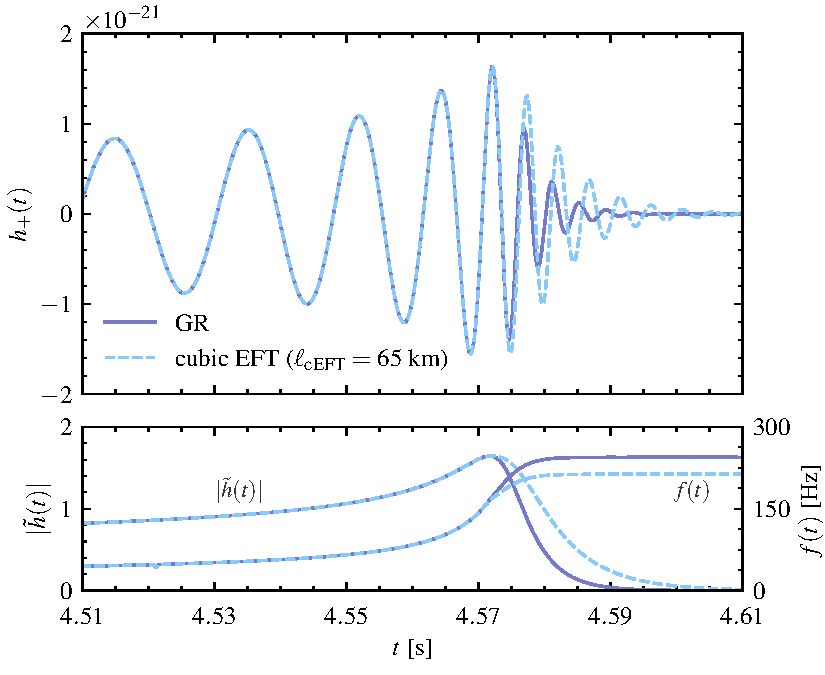
\includegraphics[width=\columnwidth]{figs/example_waveform_cubicEFT.pdf}
\caption{(Color online).~Example GW signal with GW1509140-like parameters
for both GR (solid line) and cubic EFT of GR (dashed line) with the leading-order
$n=0$ modifications to the fundamental QNM, for $\ell_{\rm cEFT} = 65$~km.
%
The former is computed with the \SEOB{} model, while the latter with the
\pSEOB{} model, with ringdown modifications according to the results in
Table~\ref{tab:ref_theories_qnms}.
%
Top panel: the $+$ polarization $h_{+}(t)$. Bottom panel: the GW amplitude
$|\tilde{h}(t)|$ (left axes) and the instantaneous frequency $f(t)$ (right axes).
}
\label{fig:example_waveform}
\end{figure}

% \begin{table*}[th]
% \begin{tabular}{c | c c c c c c c c}
% \hline
% \hline
% Theory & $p$ & $\delta \omega^{(0)}_{220}$ & $\delta \tau^{(0)}_{220}$ & $\delta \omega^{(1)}_{220}$ & $\delta \tau^{(1)}_{220}$ & QNM & Constraint & This work \\
% \hline
% EdGB      & 4 & 0.0107 & 0.0044 & $-$0.2480 & $-$1.101 &  \cite{Blazquez-Salcedo:2016enn,Pierini:2021jxd} & $\ell_{\rm GB} \leqslant 1.18$~km~(GW)~\cite{Lyu:2022gdr} & -- \\
% dCS       & 4 & 3.1964 & 6.3619 & 41.199 & 794.66 &  \cite{Wagle:2021tam}   & $\ell_{\rm CS} \leqslant 8.5$~km~(EM+GW)~\cite{Silva:2020acr}  & $\ell_{\rm CS} \leqslant 34.5$~km \\
% cEFT  & 4 & -0.5813  & 2.6469 & -3.8620 & 265.12 & \cite{Cano:2021myl} & \dots  & \dots \\
% qEFT  & 6 & \dots  & \dots & \dots & \dots & \cite{Cano:2021myl} & $\ell_{\rm qEFT} = \dots$~km~\cite{Sennett:2019bpc}  & \dots \\
% \hline
% \hline
% \end{tabular}
% \caption{Summary of the quasinormal modes calculations.
% %
% We summarize each theory we have considered together with: the exponent $p$ at
% which their QNM-modification enters, the corresponding modifications to the
% oscillation frequency $\delta \omega^{(i)}_{220}$ and decay time $\delta \tau^{(i)}_{220}$, the
% references from which we used the results from and the current best constraint
% (if applicable).
% %
% In these cases, the dimensionless parameters $\lambda_{\rm e,o}$ are degenerate
% with the length scale $\ell$.
% %
% }
% \label{tab:ref_theories_qnms}
% \end{table*}

%%%%%%%%%%%%%%%%%
\section{Parameter Inference}
In this section, we provide a basic outline of the Bayesian formalism we use to
infer the properties of the underlying GW signal, identify the most promising
events from the catalog of GW observations to base our analyses on, and discuss
the key insights they provide in constraining predictions of modified gravity
theories.

\subsection{Bayesian formalism}
If we assume that a GW signal observed in detector data $d$ is accurately
described by our waveform model \pSEOB{}, we can infer the parameters of the
model, $\bm{\lambda}$, given the hypothesis $\mathcal{H}$, using the Bayes
theorem,
%
\begin{equation}
P(\bm{\lambda} \vert d, \mathcal{H}) =
\frac{p(\bm{\lambda} \vert \mathcal{H}) \, \mathcal{L}(d \vert \bm{\lambda},\mathcal{H})}{E(d \vert \mathcal{H})}\,,
\label{eq:bayes}
\end{equation}
%
where $P(\bm{\lambda} \vert d, \mathcal{H})$ is the posterior probability distribution,
$p(\bm{\lambda} \vert \mathcal{H})$ the prior,
$\mathcal{L}(d \vert \bm{\lambda},\mathcal{H})$ the likelihood, and
$E(d \vert \mathcal{H})$ the evidence.
%
The set of parameters, $\bm{\lambda}$ is a union of the GR waveform
model parameters~$\bm{\theta}$ (c.f.  Sec.~\ref{sec:review_pSEOB}), and
$\ell$,  the only non-GR parameter in this problem which, we recall, set
the characteristic length-scale in which deviations from
GR become relevant in each of the theories described in
Sec.~\ref{sec:review_theories}. Hence,
%
\begin{equation}
\bm{\lambda} = \{\ell\} \cup \{\bm{\theta}\}.
\label{eq:def_params}
\end{equation}

% As discussed in Secs.~\ref{sec:review_theories} and \ref{sec:theory_specific_qnm}, there is a single coupling
% constants in the cases of EdGB and dCS theories, but two in the cubic and
% quartic EFTofGR.
% %
% We also hold the other beyond-GR parameters, $\{\delta \omega_k^{(j)}\},$ and $\{\delta \tau_k^{(j)}\}$
% fixed to theory-specific predictions. Hence, our set of beyond--GR parameters only includes the parameter $\{\ell \}$.
% %

Assuming stationary Gaussian noise, we can write the (log) likelihood function as,
%
\begin{equation}
\ln \mathcal{L}(d \vert \bm{\lambda},\mathcal{H}) \propto
- \tfrac{1}{2}
\langle
d - h(\bm{\lambda}) \vert d - h(\bm{\lambda})
\rangle\,,
\end{equation}
%
with noise-weighted inner product $\langle \cdot | \cdot \rangle$ defined as,
%
\begin{equation}
\langle A | B \rangle =
\int_{f_{\rm low}}^{f_{\rm high}} \, \dd f \,
\frac{\tilde{A}^{\ast}(f) \tilde{B}(f) + \tilde{A}(f) \tilde{B}^{\ast}(f)}{S_{n}(f)}\,,
\end{equation}
%
where $\tilde{A}(f)$ is the Fourier transform of $A(t)$, the asterisk denotes
complex conjugation and $S_{n}(f)$ is the power spectrum density of the
detector.
%
Assuming a specific prior distribution for our parameters (discussed further in the subsequent section), we stochastically
sample over the parameter space using a Markov-Chain Monte Carlo algorithm as implemented in
\texttt{LALInferenceMCMC}~\cite{Rover:2006ni,vanderSluys:2008qx},
a package part of the \texttt{LALInference} software suite~\cite{Veitch:2014wba,lalsuite}.
%
We subsequently marginalize over the remaining parameters to obtain the
posterior probability distribution function~(PDF) on $\ell$,  $P_j(\ell \vert d_j,\mathcal{H})$, our main parameter of interest.
%
% An example of this is shown in Fig. XX.

For $N$ independent GW observations $\{d_j\}$, $j=1,...,N$, each characterised by a posterior probability distribution $P_j(\ell \vert d_j,\mathcal{H})$, the joint posterior can be written as:
%
\begin{equation}
P(\ell | \{d_j\}) = p(\ell) \prod_{j=1}^{N} \frac{P_j(\ell | d_j)}{p_j(\ell)}\,.
\label{eq:cumulative_dist_ell}
\end{equation}
%
where $p_j(\ell)$ are the priors used for each observation, and $p(\ell)$ is an overall prior.
%
Since we assume a uniform prior on $\ell$, the joint posterior is identically
equal to the joint likelihood.
%
In some cases, we found it necessary to work with different prior ranges across
different events, within the context of a given theory.
%
In this situation, when combining the posteriors we use chose as our overall
prior the widest one among the individual events.

\subsection{Priors}

The prior probability distribution functions on the GR parameters are assumed to be uniform over the component masses, $(m_1, m_2)$, isotropically distributed on a sphere in the sky for the source location with $p(d_L) \propto d_L^2$, and isotropic on the binary orientation, $p(\iota, \psi, \phi_0) \propto \sin\iota$. For the spins $(\chi_1, \chi_2)$, we assume a prior uniform and isotropic in the spin magnitudes and restrict ourselves to the $z$-components.
This spin-prior choice can be specified in \texttt{LALInference} using the option \texttt{alignedspin-zprior}.
%
The prior on $t_0$ is uniform and its range is informed by our detection pipelines.

Among our beyond-GR parameters, $\{\ell, \delta \omega_k^{(n)}\delta \tau_k^{(n)}\}$,
as already mentioned in the previous section, we hold $\{\delta \omega_k^{(n)}\}$
and $\{\delta \tau_k^{(n)}\}$ fixed to theory-specific predictions, and allow only $\ell$
to freely vary.
%
For such cases, we assume a prior uniform between appropriate ranges on $\ell$,
making sure that our marginalized posterior distributions on $\ell$ do not rail
over the maximum prior value on $\ell$.


\subsection{Event selection}

\begin{figure}[t]
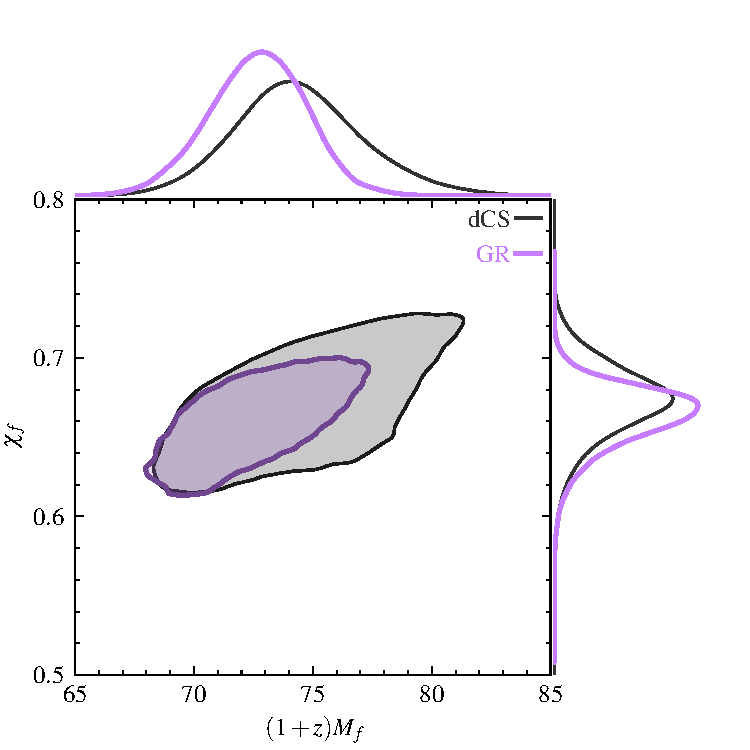
\includegraphics[width=0.9\columnwidth]{figs/tmp_GW150914_intrinsic_params_remnant.pdf}
\caption{(Color online).~Corner plot showing that the inferred final spin $\chi_f$,
detector-frame remnant mass $(1 + z) \, M_f$ for GW150915, using the same waveform model,
but without (blue contours) and with the non-GR parameters different from zero (orange contours, for
dCS gravity and $j=0$). The contours represent 90\% credible regions.
%
We see that the introduction of the non-GR parameters does not bias the
inference on the source parameters.
}
\label{fig:corner_plot}
\end{figure}

The \pSEOB{} model, as described in Sec.~\ref{sec:review_pSEOB}, is an
\emph{IMR} model which infers the properties of the underlying GW signal,
including (independently) its ringdown properties, using the Bayesian formalism
above. Naturally, the most promising candidates for our analyses are high-mass
\emph{and} loud GW observations with a significant signal-to-noise ratio (SNR)
in the post-merger part of the signal.
%
The latest LVK GW catalog~\cite{LIGOScientific:2021djp} reported 90 observed
signals not all of which are relevant for a BH ringdown analysis. In fact, in
an accompanying paper~\cite{LIGOScientific:2021sio}, the \textsc{pSEOBNRv4HM}
analysis\footnote{See, in particular, Sec.VIII A.2
in~\cite{LIGOScientific:2021sio}}, which is most similar to the \pSEOB{} model
presented in this paper, identified two events which provided the strongest
bounds on measurements of the dominant $(220)$ QNM --
GW150914~\cite{LIGOScientific:2016aoc} and
GW200129~\cite{LIGOScientific:2021djp}.
%
These two events, with a total mass of $XX \Mo$ and $XX \Mo$ respectively, are
extremely similar in their source properties. These are also two of the loudest
BBH signals observed to date with a total network SNR of XX and XX
respectively.
%
Moreover, and what is more relevant for our analysis, is their post-inspiral
(merger-ringdown) SNRs, which at XX and XX respectively (see the columns for
$\rho_{\text{post-insp}}$ in Table III of~\cite{LIGOScientific:2019fpa} and
Table IV of~\cite{LIGOScientific:2021sio}).
%
In this paper, we are going to focus on these two GW events as our probes of
the BH ringdown in modified theories of gravity.

The parameter inference in this paper follows configurations identical to the
ones used on these events for the \textsc{pSEOBNRv4HM} analysis in
Ref.~\cite{LIGOScientific:2021sio}. GW150914 was a 2-detector event (HL) while
GW200129 was 3-detector (HLV).
%
We consequently use the same strain data $h(t)$, detector
power-spectral-densities $S_n(f)$ and calibration envelopes as were used for
the analyses in Ref.~\cite{LIGOScientific:2021sio}.
%
The only difference between the sampling configurations is that we do not
sample over the fractional deviations in the $(220)$ QNM frequencies and
damping times, but instead on $\ell$ while holding $\{\delta \omega_k^{(j)}\},$
and $\{\delta \tau_k^{(j)}\}$ fixed to theory-specific predictions.
%
In the section to follow, we enumerate through the different theories and
outline the highlight results. Whenever possible, we also combine results from
multiple events to obtain the strongest possible bound on $\ell$.

% -----------------
% Corner plots here
% -----------------

As a first test ...
\hs{Move to an appendix.}

\subsection{General remarks on the interpretation of our results}
\label{sec:remarks}

There are two conditions that we must take into account before
we can confidently claim to have placed a constraint, within our model's assumptions,
with our parameter estimation study.

First, as we explained in Sec.~\ref{sec:review_theories}, all theories that we
consider must be considered as an effective field theory, meaning it should be
considered valid only below an energy scale, or equivalently, a length scale.
%
As a cut-off length scale for the validity of the EFT we use,
%
\begin{equation}
\Lambda_{\rm EFT} (\varepsilon, \mathfrak{m}) = \varepsilon \, G \mathfrak{m} / c^2 \,,
\label{eq:def_cutoff}
\end{equation}
%
where $\varepsilon$ is a dimensionless number and $\mathfrak{m}$ is the median
value of one of the mass scales involved in the problem.
%
We also momentarily restored factors of $c$ and $G$ to emphasize that $\Lambda_{\rm EFT}$ has
dimensions of length and hence can be compared to the coupling strength $\ell$.
%
In Refs.~\cite{Nair:2019iur,Perkins:2021mhb,Lyu:2022gdr}, $\varepsilon = 1/2$ was used,
but here we consider $\varepsilon \in [0, 1]$.
%
We will say that a bound has been placed on $\ell$, if most of the support of
the posterior distribution function $P(\ell)$ is in the interval
$[0, \, \Lambda_{\rm EFT}(\varepsilon, \mathfrak{m})]$.
%
In practice, this can be quantified through the cumulative distribution function
(CDF) associated with the marginalized posterior distribution $P(\ell)$,
%
\begin{equation}
P(\ell \leqslant \ell_{\rm max}) = \int_{-\infty}^{\,\ell_{\rm max}} P(\ell') \, \dd \ell'\,.
\label{eq:def_cdf}
\end{equation}
%
For instance, we will demand that for a bound with 90\% credibility to be meaningfully placed that
up to $\ell_{\rm max} = \Lambda_{\rm EFT}$ we have,
%
\begin{equation}
% \textrm{CDF}(\ell) \leqslant \textrm{CDF}(T_{\rm EFT}(\varepsilon; \, \mathfrak{m})).
P(\ell \leqslant \Lambda_{\rm EFT}) \leqslant 0.9 \,,
\quad \textrm{(EFT bound)},
\label{eq:eft_bound}
\end{equation}
%
and likewise for other credibility percentiles.

Second, as already emphasized in Ref.~\cite{Maselli:2019mjd}, the ParSpec
formalism is by construction perturbative. This means that the non-GR
deformation parameters are small, that is,
%
\begin{equation}
\gamma \, \delta \omega^{(n)} \ll 1 \,,
\,\, \textrm{and} \,\,
\gamma \, \delta \tau^{(n)} \ll 1 \,, \quad \textrm{(ParSpec bound)},
\label{eq:parspec_bound}
\end{equation}
%
for all orders $n$ in the expansion in dimensionless spin $\chi$ and where $\gamma$
is given by Eq.~\eqref{eq:def_gamma}.
%
We will also construct posterior distributions for these parameters and check if
most of their support is concentrated to a domain with values much smaller than
unity.

Another question we must consider is the following: what is the mass $\mathfrak{m}$ that we should use
in Eq.~\eqref{eq:def_cutoff}?
%
In Refs.~\cite{Nair:2019iur,Perkins:2021mhb,Lyu:2022gdr}, which attempted to
constrain dCS and shift-symmetric sGB theories with the \emph{inspiral} part of
the GW signal alone, it was natural to chose the secondary's mass $m_2$ as the most
conservative choice, since it is (by definition) the smallest mass and hence
places the lowest cut-off scale $\Lambda_{\rm EFT}$ for the validity of either of these theories as an EFT.

In our problem, the answer is not as clear. On the one hand, since we are
interested in the ringdown part of the signal, it is natural to use the
final mass $M_f$ to compute $\Lambda_{\rm EFT}$.
%
On the other hand, one may argue that the modified gravity theory under study
should be able to predict a full inspiral, merger, and ringdown of the black
hole binary before we can even make such a test, and thus the same, more conservative choice
$\gm = m_2$ should be used.
%
Here we adopt an agnostic view to this question and consider \emph{both} masses, $m_2$ and $M_f$, to
determine $\Lambda_{\rm EFT}$. We will then compare how different assumptions
yield to different interpretations of the results of our parameter estimations.


\iffalse
\subsection{Stacking posteriors}
\label{sec:stack}

If, for each event, we find that the constraints~\eqref{eq:eft_bound}
and~\eqref{eq:parspec_bound} are satisfied, we further combine the individual
posteriors distribution on $\ell$, allowing us to place a stronger bound on this parameter.
%
Let us review how do we calculate this \emph{cumulative posterior distribution} on $\ell$.

% 1. Description of data and assumption o \ell being shared
Suppose we have a data set $\{d_{i}\}$ of $N$ events which is described by
model parameters $\bm{\lambda}_{i}$, where $i$ labels each event.
%
We assume that the value of the coupling constant $\ell$, given a specific theory,
is common to all events.
%
% 2. Define joint posterior
%
The joint posterior for the parameters $\bm{\lambda}_{i}$, that describe the
data $\{d_{i}\}$, is
%
\begin{equation}
P(\ell, \{\btheta_i\} | \{d_{i}\})
= \frac{ P(\ell, \{\btheta_i\}) \, P( \{d_i\} | \ell_i, \{\btheta_i\} ) }{ P(\{d_i\}) }.
\label{eq:def_joint_posterior}
\end{equation}
%
where we separated $\ell$ from the GR waveform model parameters $\btheta$ [cf.~Eq.~\eqref{eq:def_params}].
%
% 3. Marginalisation to obtain the cumulative posterior
%
To obtain the cumulative posterior distribution on $\ell$, we marginalize
the joint posterior~\eqref{eq:def_joint_posterior} over
all parameters $\{ \btheta_i \}$, i.e.,
%
\begin{align}
P(\ell | \{d_i\}) &= \int \dd \{\btheta_i\} \, P(\ell, \{\btheta_i\} | \{d_{i}\}),
\nonumber \\
                  &= \int \dd \{\btheta_i\} \, \frac{ P(\ell, \{\btheta_i\}) \, P( \{d_i\} | \ell_i, \{\btheta_i\} ) }{ P(\{d_i\}) },
\nonumber \\
                  &= \frac{P(\ell)}{P(\{d_i\})} \int \dd \{\btheta_i\} \, P(\{\btheta_i\}) \, P( \{d_i\} | \ell, \{\btheta_i\} ),
\end{align}
%
where we have assumed that the prior on $\ell$, $P(\ell)$, is independent of
the other parameters $\{\btheta_i\}$.
%
This allow us to write $P(\ell, \{\btheta_i\} = P(\ell) P(\{\btheta_i\})$
and then move $P(\ell)$ out of the integral
%
We also moved out integral the evidence $P(\{d_i\})$, which is a normalization constant.
%
% 4. Factor the integrals in a product due to statistical independence
%
We can now factor the probabilities inside the integral, since each event is independent from another:
%
\begin{equation}
P(\ell | \{d_i\}) = \frac{P(\ell)}{P(\{d_i\})}
\prod_{i=1}^{N}
\int \dd \btheta_i \, P(\btheta_i) \, P( d_i | \ell_i, \btheta_i ).
\end{equation}
%
% 5. Final formula
We can now identify the integral as the marginalized likelihood for each individual event
%
\begin{equation}
P(\ell | \{d_i\}) = \frac{P(\ell)}{P(\{d_i\})}
\prod_{i=1}^{N} P( d_i | \ell_i ),
\end{equation}
%
which we can rewrite as
%
\begin{align}
P(\ell | \{d_i\}) &= \frac{P(\ell)}{P(\{d_i\})}
\prod_{i=1}^{N} \frac{P(d_i)}{P(\ell_i)} P(\ell_i | d_i)
\nonumber \\
&= P(\ell)
\prod_{i=1}^{N} \frac{P(\ell_i | d_i)}{P(\ell_i)}.
\label{eq:cumulative_dist_ell}
\end{align}
%
by using Bayes' theorem in the first line and cancelling the evidences in the
second line. This is our final result.

%
\hs{Abhirup, maybe move this to the subsection on priors?}
In our parameter estimation runs that we had to adjust our prior on $\ell$ depending on which event and
on which theory we examined.
%
The reasons are twofold.
%
% Describe problem 1
%
First, we found that depending on the source parameters $\btheta$,
large values of $\ell$ could result in unphysical waveforms in the frequency
band we considered. More specifically, these waveforms have a ringdown which is
considerable longer than the inspiral-merger part in the detector frequency band.
%
The fact that our sampled over these waveforms is perhaps not surprising,
because, after all, we are by construction adding corrections to the GR QNM
which \emph{increase} the damping timescale.
%
In practice, we found that these edge-cases were problematic to deal with
\texttt{LALInferenceMCMC}.
%
We overcome this problem, we reduced the prior upper-value of our prior on $\ell$.
%
This choice does not pose a problem to our parameter estimations, because these
waveforms differ grossly from the data and thus have negligible likelihood.
%
% Describe problem 2
%
However, we cannot reduce the prior on $\ell$ too much. If we do so,
to the marginalized posterior distribution on $\ell$ would rail against
the prior or, in a more extreme case, even be a uninformative, flat posterior.
%
% Summary
%
Altogether, this means that the priors $P(\ell)$ are not shared between events and
they must be taken into account when calculation the cumulative posterior function~\eqref{eq:cumulative_dist_ell}.

Finally, we use one of the approaches of Ref.~\cite{Perkins:2021mhb} to
compute the product in Eq.~\eqref{eq:cumulative_dist_ell}.
%
It method relies on first obtaining a kernel density estimator (KDE) for
the posterior distribution on $\ell$ for each individual event.
%
(See also Refs.~\cite{DelPozzo:2011pg,Cardenas-Avendano:2019zxd,Carullo:2021dui}.)
%
Next, we multiply these posteriors according to Eq.~\eqref{eq:cumulative_dist_ell}.
%
This approach based on the KDE can have difficulties in dealing with hard cut-offs in the
distribution, such as the one we impose at $\ell = 0$. We address this issue as
done in Ref.~\cite{Perkins:2021mhb}, by first doubling our number of samples as
$\{ s_i \} \cup \{ - s_i \}$, i.e., mirroring the samples across $\ell = 0$.
%
We then renormalize the associated KDE numerically in the range $\ell = [0, \infty]$.
\fi



%%%%%%%%%%%%%%%%%%%%%%%%%%%%%%%%%%%%%%%%%
\section{Results using LIGO-Virgo events}
\label{sec:results}
%%%%%%%%%%%%%%%%%%%%%%%%%%%%%%%%%%%%%%%%%

% ----------------------------------------------------------
% \hs{Convention: us 90\% credibility for the final bounds.}
% ----------------------------------------------------------

% -----------------
% Explain threshold
% -----------------


% \hs{Note to ourselves: as mentioned in~\cite{Maselli:2019mjd}:
% %
% ``As customary in parametrized approaches, we focus on perturbative corrections by assuming $\gamma_{i} \delta \omega^{(n)} \ll 1$, $\gamma_{i} \delta \tau^{(n)} \ll 1$ and GR is recovered in the limit $\gamma_{i} \to 0$.''
% We should check this \emph{in addition} to the small-coupling approximation to argue whether we placed a bound or not.
% }

\subsection{Einstein-dilaton-Gauss-Bonnet gravity}
\label{sec:results_edgb}

We start by showing our results for EdGB gravity.
%
In Fig.~\ref{fig:edgb_exec_sum} we show the marginalized posteriors of the
coupling constant $\ell_{\rm GB}$, for GW150914 (top panel) and GW200129
(middle panel), with and without the spin corrections to the $(2,2,0)$ QNM.
%
The bottom panel panel shows the joint posterior combining both events.
%
We see that for both events events, the $N_{\rm max} = 0$ posteriors are
characterized by a peak away from zero.
%
This does not mean that we are inferring a deviation from GR from data.
%
Recall that the deviations from GR in the ParSpec framework are controlled
by $\gamma$, which here reads,
%
\begin{equation}
    \gamma_{\rm GB} = \left(\frac{c^2 \ell_{\rm GB}}{ G M_{\rm s}}\right)^4\,.
\end{equation}
%
As shown in Fig.~xxx, $\gamma_{\rm GB}$ does indeed have a posterior
distribution with largest support at zero, indicating consistency between data
and GR.
%
We also observe that the inclusion of the spin corrections (i.e., curves with $N_{\rm max} = 1$)
displaces the posteriors distributions towards smaller values of $\ell_{\rm GB}$.

\begin{figure}[t]
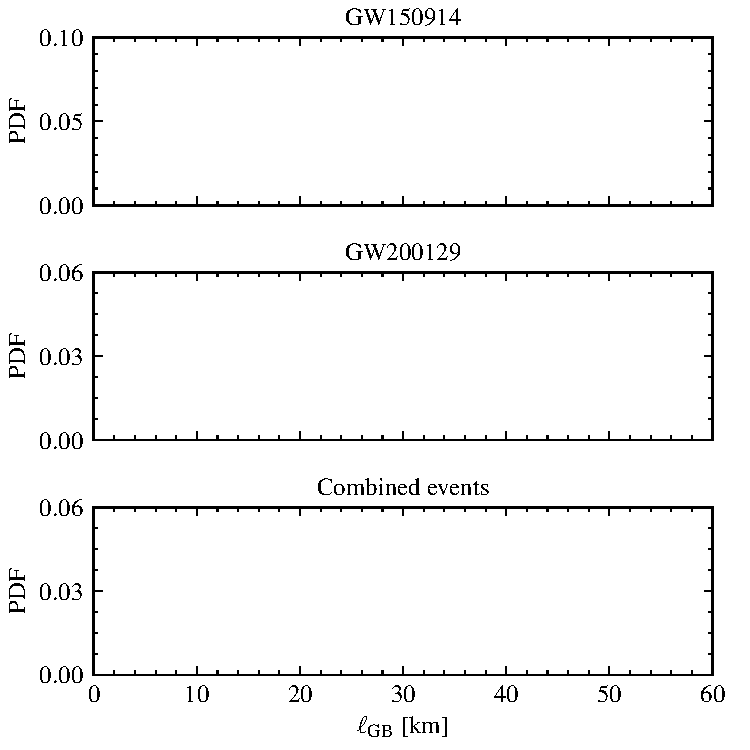
\includegraphics[width=\columnwidth]{figs/edgb_posteriors_combined.pdf}
\caption{(Color online).~Posterior distribution function in EdGB gravity
for the coupling constant $\ell_{\rm GB}$ for GW150914 (top panel), GW200129 (middle panel)
and combined events (bottom panel).
%
In all panels, different line colors correspond to the inclusion ($N_{\rm max} = 1$) or not ($N_{\rm max} = 0$)
of the linear-in-spin QNM correction.
%
The joint posteriors are shown for illustrative purposes only. As we explain in Fig.~\ref{fig:edgb_cdf} and
in the main text, our analysis of these events fails to satisfy the EFT bound~\eqref{eq:eft_bound}.
}
\label{fig:edgb_exec_sum}
\end{figure}

\begin{figure}[t]
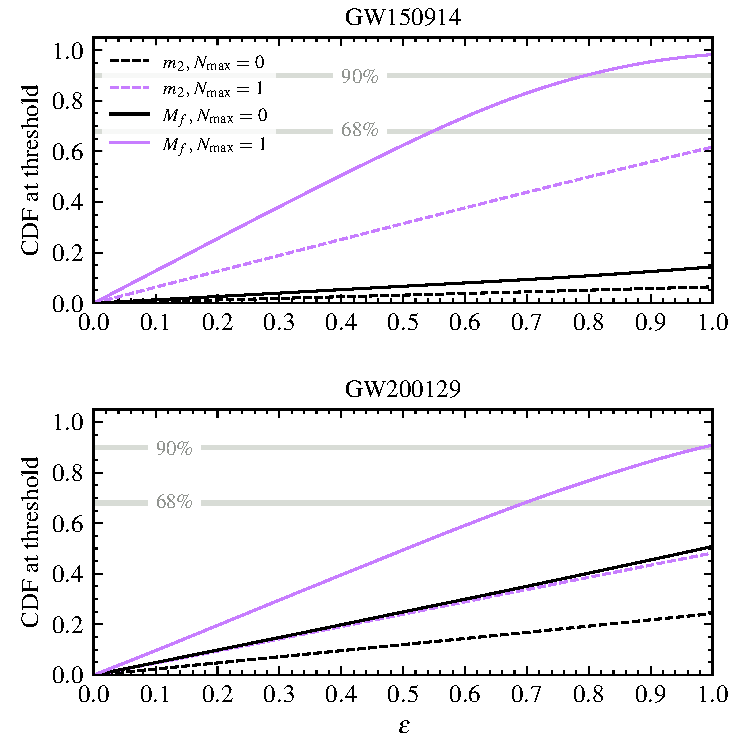
\includegraphics[width=\columnwidth]{figs/edgb_cdf_varying_threshold.pdf}
\caption{(Color online).~The cumulative distribution function evaluated at the
cut-off $\Lambda_{\rm EFT}(\varepsilon,\gm)$ EdGB gravity as a function of the parameter
$\varepsilon$ for both (dashed curves) $\gm = m_2$, the secondary's source
mass, and (solid curves) $\gm = M_{f}$, the remnant's source mass, without
(black curves) and with (purple curves) linear in spin QNM corrections. The
horizontal lines lay at 0.68 and 0.90. We see that in no situation the curves pass
through the 0.68 or 0.90 lines even at $\varepsilon = 1$. This means that no bound on $\ell_{\rm GB}$
can be placed with the events we analyzed.
}
\label{fig:edgb_cdf}
\end{figure}

\begin{table}[h]
\begin{tabular}{l l c c c}
\hline
\hline
$N_{\rm max}$ & Event &  EFT    & ParSpec & Constraint      \\
              &       &  bound? & bound?  & ($\gm = M_{f}$) \\
\hline
  & GW150914 & No  & Yes & -- \\
0 & GW200129 & No  & Yes & -- \\
  & Combined & --  & Yes & -- \\
\hline
  & GW150914 & No  & Yes & -- \\
1 & GW200129 & No  & Yes & -- \\
  & Combined & --  & Yes & -- \\
\hline
\hline
\end{tabular}
\caption{Detailed summary of our results for EdGB gravity for GW150914, GW200129, and
combined events using $\gm = M_{f}$, $\varepsilon = 1/2$ and quoting only 90\% credible results.
%
We find that we cannot place any constraint on $\ell_{\rm GB}$ with our waveform model from either GW event.
}
\label{tab:summary_edgb}
\end{table}

As we emphasized in Sec.~\ref{sec:remarks}, before drawing any conclusions on
the allowed values for $\ell_{\rm GB}$ from our parameter estimations, we
must first check whether the ``EFT''~\eqref{eq:eft_bound} and
``ParSpec''~\eqref{eq:parspec_bound} bounds are satisfied.
%
We check the validity of the EFT bound in Fig.~\ref{fig:edgb_cdf}. In the top (bottom) panel we show
the cumulative density function of the $\ell_{\rm GB}$ posteriors for GW150914 (GW200129), obtained
evaluating the integral~\eqref{eq:def_cdf} with $\Lambda_{\rm EFT}(\varepsilon, \mathfrak{m})$,
with the mass scale set by the secondary's mass (i.e., $\mathfrak{m} = m_2$, dashed lines) or
the remnant's mass ($\mathfrak{m} = M_f$, solid lines), while varying $\varepsilon$ between 0 and 1.
%
For GW150914, we see that for the $N_{\rm max} = 0$ curves, that the CDF never goes
past $0.2$, regardless of the mass scale $\mathfrak{m}$ used and even at $\varepsilon =
1$. This shows that that the ``EFT bound'' given by Eq.~\eqref{eq:eft_bound} is
never met at a significant credibility and thus that we cannot place a bound on
$\ell_{\rm GB}$.
%
The situation is similar for GW200129 with $N_{\rm max} = 0$ and does not
change for either event when we add spin corrections to the EdGB QNM.
%
Taken together we are led to \emph{conclude that we cannot constrain EdGB gravity with our
present model}.
%
We summarize our findings in Table~\ref{tab:summary_edgb}.

Let us place our results in a broader context. In particular, let us contrast
them against those of Ref.~\cite{Lyu:2022gdr} which placed the bound
%
$\ell_{\rm GB} \leqslant 1.33$~km
%
using the neutron star-black hole binaries GW200105 and GW200115~\cite{LIGOScientific:2021qlt}, and
of Refs.~\cite{Nair:2019iur,Perkins:2021mhb}, which placed the bound
%
$\ell_{\rm GB} \leqslant 1.7$~km,
%
by stacking the posterior of $\ell_{\rm GB}$ from a  selection of black hole binaries from the GWTC-1 and GWTC-2 catalogs
with at least one relatively low-mass binary component~\cite{}\footnote{These bounds
are, strictly speaking, valid only when the scalar field $\varphi$ is small, i.e., $\varphi \ll 1$, and
take into consideration only the leading-order scalar field contribution arising from the dilatonic coupling.}.
%
These works use the \emph{inspiral} portion of GW event only and a constraint
on EdGB gravity can be obtained because black holes in this theory carry a
monopole scalar charge which in turn can source dipolar scalar radiation,
that affects the GW phase at $-1$PN order, relative to the dominant GR contribution, and
is proportional to the difference between the charges of binary components.
%
Now, the magnitude of the scalar charge scales roughly with the inverse of the black hole's mass squared, that is,
smaller (larger) back holes carry large (smaller) scalar charges. Qualitatively, this is because the scalar field
is sourced by the Gauss-Bonnet curvature invariant, which is large for black holes with small masses.
%
Beyond-GR corrections to the inspiral are, by construction, not present in our
waveform model and constitutes a important ingredient to be added in forthcoming
versions of the model.
%
In addition to the larger mass (which suppresses the black hole's charge), the
QNM of EdGB gravity differ very little from GR as observed in~\cite{Blazquez-Salcedo:2016enn}.
%
Hence, here we have an example of a theory in which the inspiral portion of the signal
is more constraining then the ringdown portion of the signal.
%
As we will next, the situation is the opposite for dCS gravity.


\subsection{Dynamical Chern-Simons}
\label{sec:results_dcs}

\begin{figure}[t]
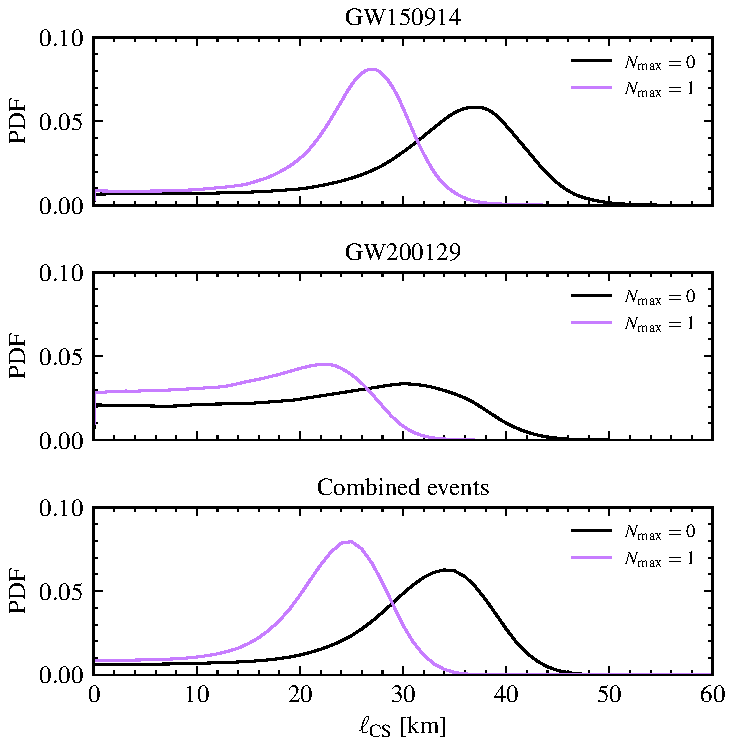
\includegraphics[width=\columnwidth]{figs/dcs_posteriors_combined.pdf}
\caption{(Color online).~Posterior distribution function for the coupling constant $\ell_{\rm CS}$ for
GW150914 (top panel), GW200129 (middle panel) and combined events (bottom panel).
%
In all panels, we use solid and dashed lines to correspond to the inclusion or not of the linear
in spin QNM correction.
%
We stress that posteriors obtained including $n=1$ corrections, violated conditions~\eqref{eq:parspec_bound}
and therefore should not be used to draw meaningful conclusions. We show them for illustrative purposes
and also to emphasize the importance of taking conditions~\eqref{eq:eft_bound} and~\eqref{eq:parspec_bound}
simultaneously into consideration when analyzing the results of the parameter estimation.
}
\label{fig:dCS_exec_sum}
\end{figure}

\begin{figure}[t]
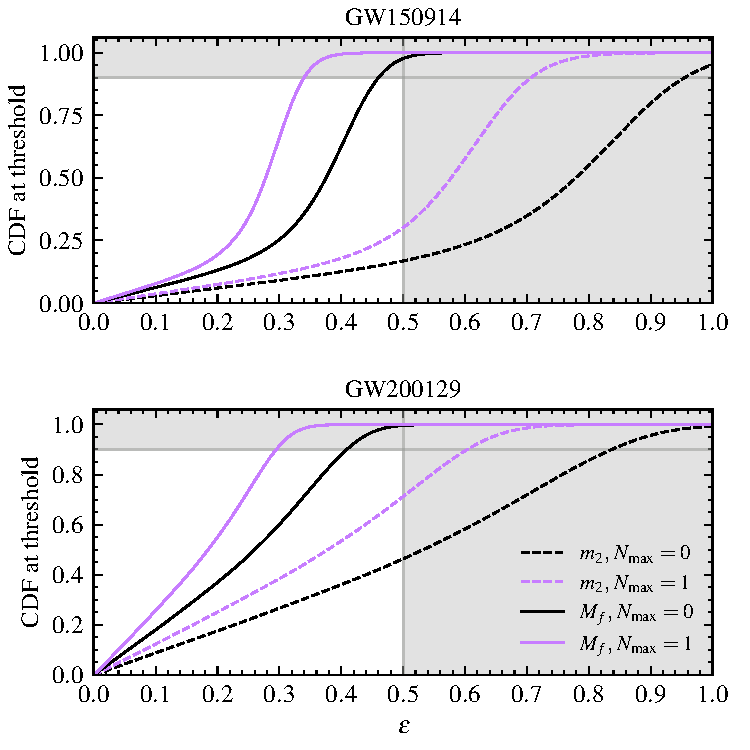
\includegraphics[width=\columnwidth]{figs/dcs_cdf_varying_threshold.pdf}
\caption{(Color online).~The cumulative distribution function evaluated at the
cut-off $\Lambda_{\rm EFT}(\varepsilon, \gm)$ as a function of the parameter $\varepsilon$ for both
$\gm = m_2$ (solid and dashed lines) and $\gm = M_{f}$ (dot-dashed and dotted lines) without
(blue lines) and with (orange lines) linear-in-spin QNM corrections.
The horizontal lines lay at 0.68 and 0.90.
%
We see that the CDF curves for $\gm = M_{f}$ are above 90\% for $\varepsilon =
1/2$ for both events, with and without including the $n = 1$ dCS corrections to
the dominant QNM.
}
\label{fig:dcs_cdf}
\end{figure}

We now turn our attention to dCS gravity.
%
In Fig.~\ref{fig:dCS_exec_sum} we show the marginalized posterior distribution
function of $\ell_{\rm CS}$ for both events GW150914 (top panel) and GW200129
(middle panel), with (dashed line) and without (solid line) spin corrections to
dominant $(2,2,0)$~QNM.
%
Perhaps the most salient feature of these posteriors is that they are not
peaked at $\ell_{\rm CS}$, which may mislead us to believe that we are seeing a
deviation from GR. This is not the case and the situation is that same as the
one we discussed in the previous section for EdGB gravity.
%
We verified that
%
\begin{equation}
    \gamma_{\rm CS} = \left( \frac{c^2 \ell_{\rm CS}}{G M_{\rm s}} \right)^{4}\,,
\end{equation}
%
does indeed peak at zero indicating consistency with GR, similarly to what is shown in Fig.~\ref{} for $\gamma_{\rm GB}$.
%
We also see that in both cases, that the inclusion leading-order-in-spin
correction to the mode, displaces the posteriors towards smaller values of
$\ell_{\rm CS}$. This can be seen more evidently by looking at the location of
posterior peaks.
%
Finally, in the bottom panel, we show the combined result for both events.

In Fig.~\ref{fig:dcs_cdf} we show the cumulative distribution function,
obtained from Eq.~\eqref{eq:def_cdf}, with $\ell_{\rm max} = \Lambda_{\rm EFT} (\varepsilon, \gm)$,
for both GW150914 (top panel) and GW200129 (bottom panel), where $\Lambda_{\rm EFT}$
is calculated with either $\gm = m_2$ (dashed lines) or $M_{f}$ (solid lines),
and in the range $\varepsilon \in [0,1]$.
%
For GW150914, we see that with $\gm = m_2$ that Eq.~\eqref{eq:eft_bound} is not
satisfied unless $\varepsilon \approx 0.9$ (with only $n=0$ corrections) and
$\varepsilon \approx 0.7$ (with both $n=0$ and $1$ corrections).
%
The situation is different if we use $\gm = M_f$. In this case, we find that
with or without spin corrections that Eq.~\eqref{eq:eft_bound} can be satisfied
with $\varepsilon \leqslant 1/2$, i.e., below the criteria used
Refs.~\cite{Nair:2019iur,Perkins:2021mhb,Lyu:2022gdr}.
%
This means that with our model's assumptions and using the remnant's source mass $M_f$ to set the
cut-off scale that we can claim an upper bound
%
\begin{equation}
\ell_{\rm CS} \leqslant 42.6~\textrm{km}
\quad \textrm{(90\% credibility)},
\end{equation}
%
on dCS gravity and would constitute the first bound on this theory with
gravitational-wave observations alone.
%
We also note that since the CDF grows fast in approximate domain $\varepsilon = [0.2, 0.4]$,
that a stronger, albeit at lower credibility,
%
\begin{equation}
\ell_{\rm CS} \leqslant 37.4~\textrm{km}
% ~( = \Lambda_{\rm EFT}(0.3, M_{f}) )
\quad \textrm{at 68\% credibility},
\end{equation}
%
can also be placed, when $N_{\rm max}=0$.

We can draw qualitatively similar conclusions from the GW200129 event.
In particular, we find,
%
\begin{equation}
\ell_{\rm CS} \leqslant 36.6~\textrm{km}
% 43.9~\textrm{km}~( = \Lambda_{\rm EFT}(\tfrac{1}{2}, M_{f}) )
\quad \textrm{(90\% credibility)},
\end{equation}
%
and
%
\begin{equation}
\ell_{\rm CS} \leqslant 29.1~\textrm{km}
% ~( = \Lambda_{\rm EFT}(0.3, M_{f}) )
\quad \textrm{(68\% credibility)},
\end{equation}
%
when $N_{\rm max}=0$.
%
These stronger bound are a consequence of the larger support for $\ell_{\rm CS} \lessapprox 15$~km
for GW200129 (compare the top and middle panels in Fig.~\ref{fig:dCS_exec_sum}), and in part due to
the smaller median remnant ($M_{f} \approx 59.5\msun$ versus $M_{f} \approx 61.8\msun$ for GW150914).

We also found for both GW events, that the
perturbative-conditions~\eqref{eq:parspec_bound} required by the ParSpec
formalism is violated for the $\gamma_{\rm CS} \, \delta \tau^{(1)}$ coefficient.
%
This means that we cannot use these posterior to infer any meaningful bound on dCS gravity
and that is why we quoted only the $N_{\rm max}=0$ bound above.

Finally, since both event individually led to a bound on $\ell_{\rm CS}$
(assuming a cut-off scale for $\gm = M_{f}$ and $j = 0$), we can combine the
posteriors to obtain the cumulative bound,
%
\begin{equation}
\ell_{\rm CS} \leqslant 38.7~\textrm{km}
\quad \textrm{(90\% credibility)},
\end{equation}
%
which is the main result of this section.
%
This bound is approximately a factor of four weaker than that placed by
Ref.~\cite{Silva:2020acr}, but
%
(i) relies only on GW observations and
%
(ii) suggests that a ringdown analysis can potentially place constraints on
theories which evade GW tests using inspiral information alone, such as the
case of dCS gravity~\cite{Nair:2019iur,Perkins:2021mhb,Lyu:2022gdr}.
%
In Table~\ref{tab:summary_dcs} we summarize our findings of this section.

\begin{table}[h]
\begin{tabular}{l l c c c}
\hline
\hline
$N_{\rm max}$ & Event & EFT    & ParSpec & Constraint ($\gm = M_{f}$) \\
              &       & bound? & bound?  &                            \\
\hline
%       & GW150914 & Yes & Yes & $\ell_{\rm CS} \leqslant 46.5$~km \\
% 0     & GW200129 & Yes & Yes & $\ell_{\rm CS} \leqslant 43.9$~km \\
%       & Combined & Yes & Yes & \cellcolor{blue!10}$\ell_{\rm CS} \leqslant 34.5$~km \\
      & GW150914 & Yes & Yes & $\ell_{\rm CS} \leqslant 41.9$~km \\
0     & GW200129 & Yes & Yes & $\ell_{\rm CS} \leqslant 35.8$~km \\
      & Combined &     &     & \cellcolor{black!10}$\ell_{\rm CS} \leqslant 38.7$~km \\
\hline
      & GW150914 & Yes & No  & --                                 \\
1     & GW200129 & Yes & No  & --                                 \\
      & Combined &     &     & --                                 \\
\hline
\hline
\end{tabular}
\caption{Detailed summary of our results for dCS gravity for GW150914, GW200129, and
combined events using $\gm = M_{f}$, $\varepsilon = 1/2$ and quoting only 90\% credible results.
%
We found that while our posteriors satisfy the condition~\eqref{eq:eft_bound} (with $\varepsilon = 1/2$),
they do not obey the condition~\eqref{eq:parspec_bound} for $j = 1$. This means
that our results for $N_{\rm max}=0$ are the only ones we can confidently quote.
%
The combined bound, which is also quoted in Table~\ref{tab:ref_theories_qnms},
is $\ell_{\rm CS} \leqslant 38.7$~km.
}
\label{tab:summary_dcs}
\end{table}

\subsection{cubic effective-field-theory of general relativity}
\label{sec:results_ceft}

\begin{figure}[t]
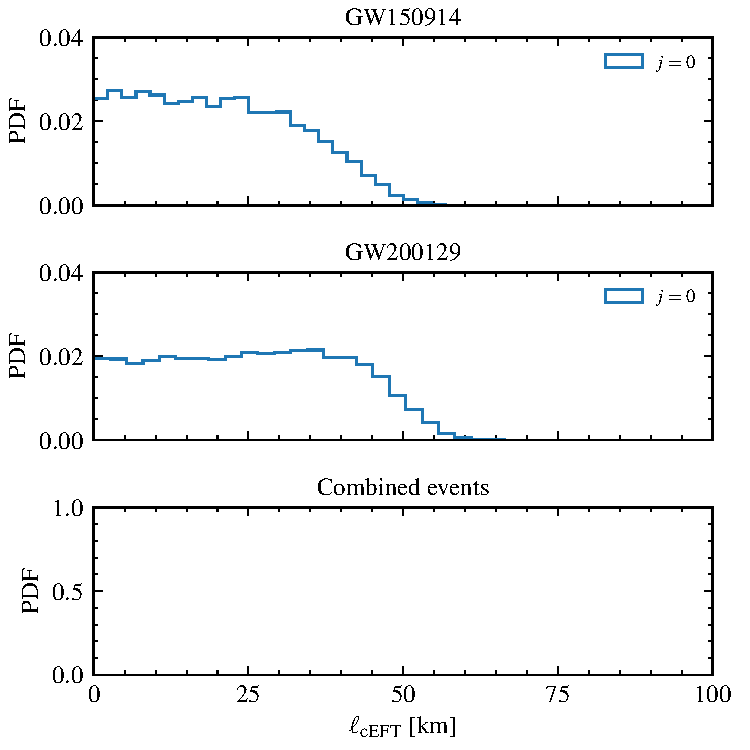
\includegraphics[width=\columnwidth]{figs/ceft_posteriors_combined.pdf}
\caption{(Color online).~Posterior distribution function for the coupling constant $\ell_{\rm cEFT}$ for
GW150914 (top panel), GW200129 (middle panel) and combined events (bottom panel).
%
In all panels, we use solid and dashed lines to correspond to the inclusion or not of the linear
in spin QNM correction.
%
\hs{TODO}
}
\label{fig:cEFT_exec_sum}
\end{figure}

\begin{figure}[t]
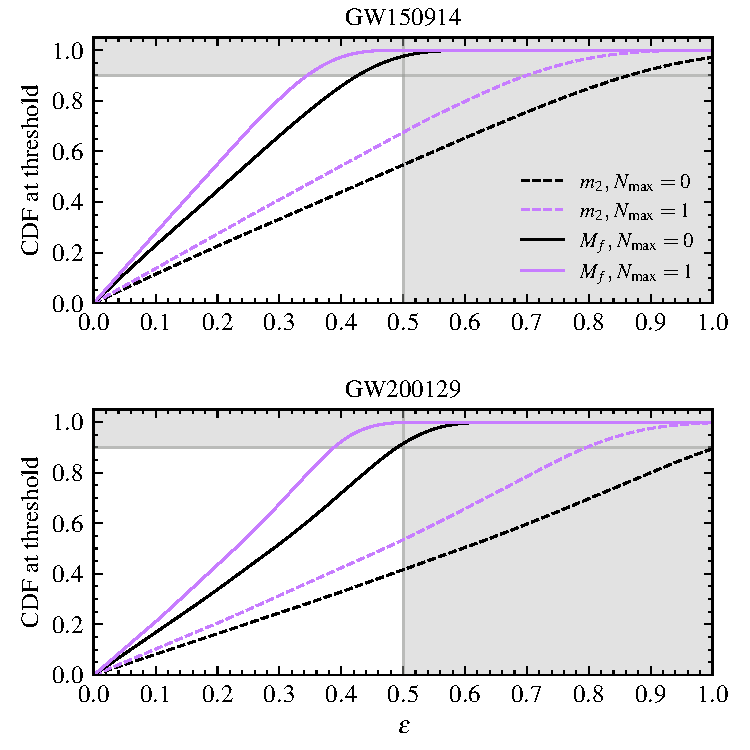
\includegraphics[width=\columnwidth]{figs/ceft_cdf_varying_threshold.pdf}
\caption{
}
\label{fig:cEFT_cdf}
\end{figure}

\begin{table}[h]
\begin{tabular}{l l c c c}
\hline
\hline
$N_{\rm max}$ & Event & EFT    & ParSpec & Constraint ($\gm = M_{f}$) \\
              &       & bound? & bound?  &                            \\
\hline
  & GW150914  & Yes & Yes &  $\ell_{\rm cEFT} \leqslant 38.2$~km \\
0 & GW200129  & Yes & Yes &  $\ell_{\rm cEFT} \leqslant 42.5$~km \\
  & Combined  &     &     &  \cellcolor{black!10}$\ell_{\rm cEFT} \leqslant 38.2$~km \\
\hline
  & GW150914  & Yes  & No  &  -- \\
1 & GW200129  & Yes  & No  &  -- \\
  & Combined  &      &     &  -- \\
\hline
\hline
\end{tabular}
\caption{Detailed summary of our results the cubic EFT of GR for GW150914, GW200129, and
combined events using $\gm = M_{f}$, $\varepsilon = 1/2$ and quoting only 90\% credible results.
}
\label{tab:summary_ceft}
\end{table}

\subsection{quartic effective-field-theory of general relativity}
\label{sec:results_qeft}

\begin{figure}[t]
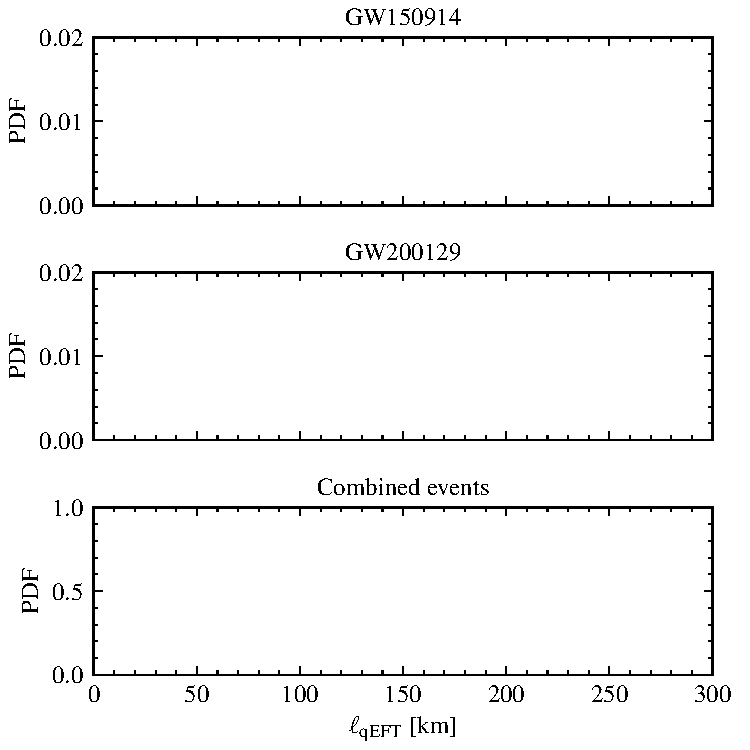
\includegraphics[width=\columnwidth]{figs/qeft_posteriors_combined.pdf}
\caption{(Color online).~Posterior distribution function for the coupling constant $\ell_{\rm qEFT}$ for
GW150914 (top panel), GW200129 (middle panel) and combined events (bottom panel).
%
In all panels, we use solid and dashed lines to correspond to the inclusion or not of the linear
in spin QNM correction.
%
\hs{TODO}
}
\label{fig:qEFT_exec_sum}
\end{figure}

\begin{figure}[t]
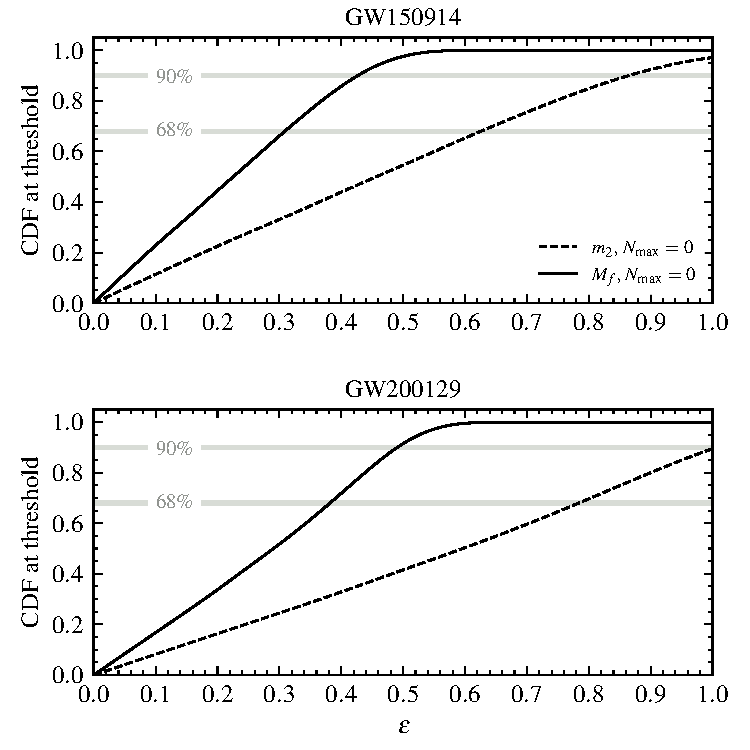
\includegraphics[width=\columnwidth]{figs/qeft_cdf_varying_threshold.pdf}
\caption{
}
\label{fig:qEFT_cdf}
\end{figure}

\begin{table}[h]
\begin{tabular}{l l c c c}
\hline
\hline
$N_{\rm max}$ & Event & EFT    & ParSpec & Constraint ($\gm = M_{f}$) \\
              &       & bound? & bound?  &                            \\
\hline
  & GW150914 & Yes & Yes  & $\ell_{\rm qEFT} \leqslant 51.7$~km \\
0 & GW200129 & Yes & Yes  & $\ell_{\rm qEFT} \leqslant 54.8$~km \\
  & Combined &     &      & \cellcolor{black!10}$\ell_{\rm qEFT} \leqslant 51.3$~km \\
\hline
  & GW150914 &  &     &    \\
1 & GW200129 &  &     &    \\
  & Combined &  &     &    \\
\hline
\hline
\end{tabular}
\caption{Detailed summary of our results the quartic EFT of GR for GW150914, GW200129, and
combined events using $\gm = M_{f}$, $\varepsilon = 1/2$ and quoting only 90\% credible results.
%
\hs{Need to debug $N_{\rm max} = 1$ runs.}
%
}
\label{tab:summary_qeft}
\end{table}

% \begin{figure}[t]
% 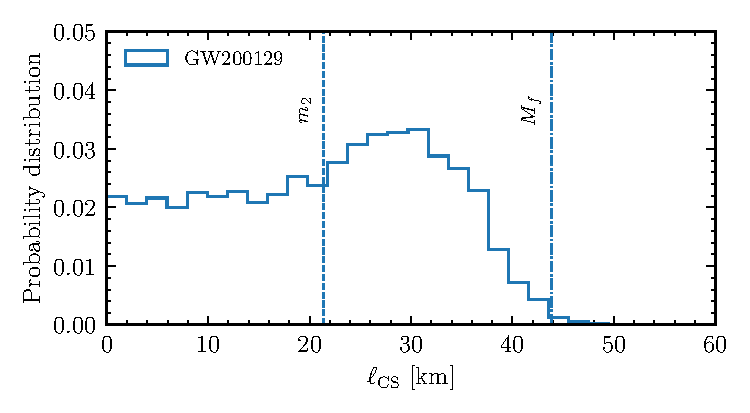
\includegraphics[width=\columnwidth]{figs/dcs_GW200129.pdf}
% \caption{Posterior probability distribution on $\ell_{\rm CS}$ with GW200129.
% The posterior shows that information was gained on this parameter relative to
% the initial uniform prior distribution $\ell_{\rm CS} \in [0,\, 200]$~km.
% %
% The vertical lines represent two threshold for the validity of the theory as
% an EFT.
% %
% The dotted line (labeled ``$m_2$'') at $\ell_{\rm CS} \approx 21.3$~km is
% given by the median value of the secondary's mass $\varepsilon \, (G m_2 / c^2)$.
% %
% The dot-dashed line (labeled ``$M_{f}$'') at $\ell_{\rm CS} \approx 43.8$~km is
% given by the median value of the remnant's mass $\varepsilon \, (G M_{f} / c^2)$.
% %
% For both, we used $\varepsilon = 0.5$.
% %
% If we take the latter as a length scale for the validity of dCS as an EFT, we
% have place upper bound on $\ell_{\rm CS} \leqslant 43.8$~km, within the
% approximation of our formalism.
% }
% \label{fig:dCS_bounds}
% \end{figure}
%
% \begin{figure}[t]
% 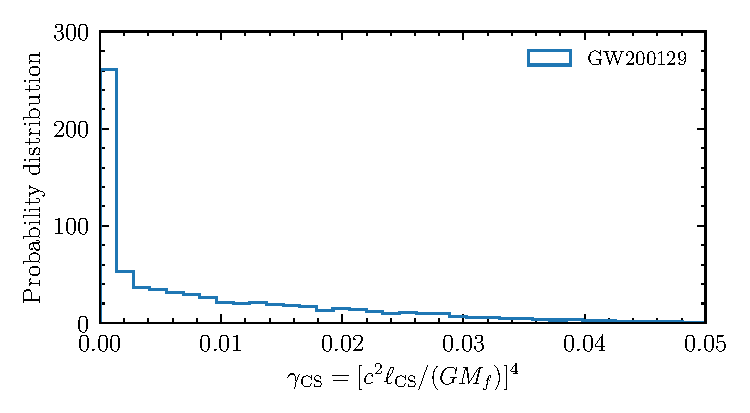
\includegraphics[width=\columnwidth]{figs/dcs_gamma_GW200129.pdf}
% \caption{Posterior probability distribution on $\gamma_{\rm CS}$ with GW200129.
% The posterior shows that the parameter $\gamma$ [see Eq.~\eqref{eq:def_gamma}]
% in dynamical Chern-Simons has a peak at zero, indicating consistency with GR.
% }
% \label{fig:dCS_gamma_plot}
% \end{figure}

%%%%%%%%%%%%%%%%%%%%%%%
\section{Conclusions}
\label{sec:conclusions}
%%%%%%%%%%%%%%%%%%%%%%%

% -------------------------------------------------------------
% \hs{Try to draw some conclusions that apply to all theories.}
% -------------------------------------------------------------

We presented an unified framework to combine the parametrized formalism introduced
to model deviations to the GR QNMs~\cite{Maselli:2019mjd} with the \pSEOB~waveform model.
%
We showed through concrete examples how theory-specific calculations QNM of
slowly-rotating BHs in modified gravity theories can be mapped upon the
theory-agnostic beyond-GR parameters of the ParSpec formalism.
%
Together this allowed us to apply the \pSEOB~waveform model to test four
modified gravity theories (EdGB, dCS, cubic, and quartic
effective-field-theories of GR) using data from the GW events GW150914 and GW200129.
%
We found, in particular that, within the assumptions of our model and by
stacking posteriors, that the coupling constant of dCS gravity is bound to
$\ell_{\rm CS} \leqslant 34.5$~km.
%
In contrast, we could place any constraint of the coupling constants in EdGB gravity $\ell_{\rm GB}$.
%
This dichotomy between these theories has an analogy with works that considered
the inspiral part of the GW signal alone.
%
In that case, it is dCS which is unconstrained, while EdGB, in principle can be
constrained, based on results for the closely related shift-symmetric version
of this theory.

Our work shows that there are theories of gravity (such as dCS) which can by-pass observational
constraints from the inspiral phase alone, {\it yet} would not, if we
analyze the ringdown.
%
We hope that our result thus serve as additional motivation for future work
modeling the late-inspiral, merger and ringdown of coalescing BHs in modified
gravity theories.

Let us discuss some avenues for future work \dots

\hs{TODO: say that we could try to expand the waveform model to include modification to
the inspiral part too; maybe through FTI~\cite{Mehta:2022pcn}?}

\hs{TODO: add that we could try to parametrize the final black hole mass and spin estimates formulas we
use at the moment~\cite{Hofmann:2016yih}. Maybe comment that a possible first attempt could follow~\cite{Buonanno:2007sv},
as done in~\cite{Jai-akson:2017ldo,Li:2020wse}. Say that ultimately we will need to informed by NR in beyond-GR.}

\hs{I suspect that by construction the $N_{\rm max} = 1$ cases will often fail to satisfy our
perturbative bounds. If so, add explanation here.}

% -----------------------------------------------------------------------------
% \hs{Say that the fact we spin correction look important reinforces the
% importance of calculation QNMs of spinning black holes beyond-GR.}
%
% \hs{Say it is important to go beyond mode calculation and actually understand
% how the QNM appear in the GW signal.}
% -----------------------------------------------------------------------------

\appendix

\section{Details of the determination of the theory-specific
ParSpec coefficients}
\label{app:map_details}

\subsection{Einstein-dilaton-Gauss-Bonnet}
\label{app:map_edgb}

\subsection{dynamical Chern-Simons}
\label{app:map_dcs}

% Let us show one concrete example of how this mapping is done.
%
In Ref.~\cite{Wagle:2021tam} the QNMs of slow-rotating BHs in dCS gravity were calculated
and it was found that the axial gravitational modes have their damping time increased as we
increase the Chern-Simons coupling $\ell_{\rm CS}$ at fixed spin $\chi$ of the BH.
%
Hence, according to the prescription of Sec.~\ref{sec:theory_specific_qnm}, this is the branch of QNMs we will select.

We can now proceed to determine $\delta\omega^{(n)}$ and $\delta\tau^{(n)}$ as follows.
%
Using the fitting formula Eq.~(54a) of~\cite{Wagle:2021tam}, namely,
%
\begin{equation}
    M \omega_{\rm CS} = c_{1} + c_{2} \kappa \zeta + (c_{3} + c_{4} \kappa \zeta) \, (1 - \chi)^{c_{5} + c_{6} \kappa \zeta},
    \label{eq:omega_dsc_eg}
\end{equation}
%
and similarly for the imaginary part ${\rm Im}(\sigma_{\rm CS}) =  - 1 / \tau_{\rm CS}$.
%
Here $\kappa = 1/(16 \pi)$, $\zeta = \ell_{\rm CS}^{4} / (M^4 \kappa)$, and thus
%
\begin{equation}
\kappa \zeta = (\ell_{\rm CS} / M)^4 \,,
\end{equation}
%
and $c_{i}$ are fitting coefficients which can be found in Ref.~\cite{Wagle:2021tam}, Table II.
%
In the context of a binary BH merger, $M$ is interpreted as the remnant mass $\Mf$.

We now expand Eq.~\eqref{eq:omega_dsc_eg} to leading-orders in $\chi$ and $\ell_{\rm CS}$, and
gather the terms proportional to $\ell_{\rm CS}$.
%
We obtain
%
\begin{align}
    \Mf \, \omega_{\rm CS} &=
    \left[ 0.3722 + 1.1945 (\ell_{\rm CS} / \Mf)^4 \right]
    \nonumber \\
    &\quad + \left[0.1861 + 5.1828 (\ell_{\rm CS} / \Mf)^4 \right] \, \chi\,,
    \label{eq:omega_dcs_interm}
\end{align}
%
where we made use of the numerical value of the coefficients $c_{i}$.
%
We find that (reassuringly) that the nonrotating GR part of the expression above agree with $\omega^{(0)}$ of Ref.~\cite{Maselli:2019mjd}
to 0.5\% relative percent error. The same error estimate is larger ($\approx 20$\%) for the linear-in-spin coefficient;
0.1861 in comparison to 0.1258 of Ref.~\cite{Maselli:2019mjd}.
%
We attribute this difference to Ref.~\cite{Wagle:2021tam} having fitted Eq.~\eqref{eq:omega_dsc_eg} to QNM data compute to linear-order in spin, whereas~\cite{Maselli:2019mjd}
fitted Eq.~\eqref{eq:kerr_expansion} to Kerr QNM valid to all orders in spin.

We can now isolate the dCS corrections from Eq.~\eqref{eq:omega_dcs_interm} and
compare against Eq.~\eqref{eq:qnm_nongr_iso}, to find
%
\begin{equation}
p_{\rm CS} = 4\,, \quad \delta \omega^{(0)}_{\rm CS} = 3.1964\,, \quad \delta \omega^{(1)}_{\rm CS} = 41.199\,.
\label{eq:cs_omega_coefs}
\end{equation}

We can carry the same steps for $\tau_{\rm CS}$ and find
%
\begin{equation}
\delta \tau^{(0)}_{\rm CS} = 6.3619\,, \quad \delta \tau^{(1)}_{\rm CS} = 794.66\,.
\label{eq:cs_tau_coefs}
\end{equation}
%
which completes the set of fixed parameters beyond-GR parameters in the ringdown of the \pSEOB{} waveform model.
%
We remark that the alarmingly large values of $\delta \omega_{\rm CS}^{(1)}$ and $\delta \tau_{\rm CS}^{(1)}$
are compensated by the assumptions that $(\ell_{\rm CS} / M_f)^2$ and $\chi$ are much less than unity. These
are the assumptions use to calculate the QNM frequencies both in Ref.~\cite{Wagle:2021tam}.

\subsection{Effective-field-theories GR}
\label{app:map_eftofgr}



%%%%%%%%%%%%%%%%%
\section*{Acknowledgements}
\label{sec:acknowledgements}
%
We thank Emanuele Berti, Andrea Maselli, Caio F. B. Macedo, Deyan Mihaylov,
Serguei Ossokine, Scott E. Perkins, and Helvi Witek for discussions.
%
We are grateful for the computational resources provided by the Max Planck
Institute for Gravitational Physics in Potsdam, specifically the
high-performace computing cluster Hypatia and to Steffen Grunewald for
assistance.
%
The authors would like to thank everyone at the frontline of the Covid-19
pandemic.
%%%%%%%%%%%%%%%%%

% \bibliographystyle{apsrev}
\bibliography{paper_alt_theor_bounds}

\end{document}
